\documentclass[preprint,12pt]{elsarticle}
\usepackage{amsmath,amssymb,amsfonts}
\usepackage{cases} 
\usepackage{lineno,hyperref}
\usepackage{cases} 
\usepackage[ruled,vlined]{algorithm2e}
% \usepackage{algorithmic}
\usepackage{capt-of}
\usepackage{flushend} %to adjust the height of two column at the last page
% \usepackage[tight,footnotesize]{subfigure}
\usepackage{caption}
\usepackage{float}
\usepackage{array}
%\usepackage{cite}
\usepackage{graphicx}
\usepackage{multirow}
\usepackage[table,xcdraw]{xcolor}
\usepackage{subcaption}
\usepackage{siunitx}
\usepackage{glossaries}
\usepackage{titlesec}
\usepackage{multirow}
\titleformat{\section}
  {\normalfont\Large\bfseries}{\thesection}{1em}{}  % Large and bold for \section
\titleformat{\subsection}
  {\normalfont\large\bfseries}{\thesubsection}{1em}{}  % Slightly smaller and bold for \subsection
\titleformat{\subsubsection}
  {\normalfont\normalsize\bfseries}{\thesubsubsection}{1em}{} 
  % Normal size and bold for \subsubsection
\setlength{\parskip}{0.5em}
% \SetAlFnt{\footnotesize}
% \SetKw{KwDownTo}{downto}
% \SetKw{KwTrue}{true}
% \SetKw{KwFalse}{false}
% \SetKwInOut{Input}{Input}
% \SetKwInOut{Output}{Output}
% \SetKw{KwAnd}{and}

% \renewcommand*{\algorithmcfname}{\footnotesize{Algorithm}}
% \newcommand{\LineIf}[2]{ \State \algorithmicif\ {#1} \algorithmicthen\ {#2} \algorithmicend\ \algorithmicif }
% \newcommand{\LINEFOR}[2]{%
% 	\STATE\algorithmicfor\ {#1}\ \algorithmicdo\ {#2} \algorithmicend\ \algorithmicfor%
% }
% \makeatletter
% \newcommand{\setword}[2]{%
%   \phantomsection
%   #1\def\@currentlabel{\unexpanded{#1}}\label{#2}%
% }
% \makeatother
% %%%%%%%%% theorem environment 
% \usepackage{amsthm}
% \renewcommand{\algorithmicrequire}{\textbf{Input:}}
% \renewcommand{\algorithmicensure}{\textbf{Output:}}
% \newcommand{\algorithmicbreak}{\textbf{break}}
% \newcommand{\BREAK}{\STATE \algorithmicbreak}
% \newcommand{\algorithmiccontinue}{\textbf{continue}}
% \newcommand{\CONTINUE}{\STATE \algorithmiccontinue}
% \renewcommand{\algorithmiccomment}[1]{// #1}

%\newcommand{\subparagraph}{}

% correct bad hyphenation here
\hyphenation{op-tical net-works semi-conduc-tor}
\usepackage{rotating}
\usepackage{placeins}
\modulolinenumbers[5]

\journal{Journal of \LaTeX\ Templates}

%%%%%%%%%%%%%%%%%%%%%%%
%% Elsevier bibliography styles
%%%%%%%%%%%%%%%%%%%%%%%
%% To change the style, put a % in front of the second line of the current style and
%% remove the % from the second line of the style you would like to use.
%%%%%%%%%%%%%%%%%%%%%%%

%% Numbered
%\bibliographystyle{model1-num-names}

%% Numbered without titles
%\bibliographystyle{model1a-num-names}

%% Harvard
%\bibliographystyle{model2-names.bst}\biboptions{authoryear}

%% Vancouver numbered
%\usepackage{numcompress}\bibliographystyle{model3-num-names}

%% Vancouver name/year
%\usepackage{numcompress}\bibliographystyle{model4-names}\biboptions{authoryear}

%% APA style
%\bibliographystyle{model5-names}\biboptions{authoryear}

%% AMA style
%\usepackage{numcompress}\bibliographystyle{model6-num-names}

%% `Elsevier LaTeX' style
%\bibliographystyle{elsarticle-num}
%%%%%%%%%%%%%%%%%%%%%%%

\hypersetup{pdfauthor=true}

\SetKw{KwTrue}{true}
\SetKw{KwFalse}{false}
\SetKw{KwAnd}{and}
\SetKw{KwOr}{or}
\SetKw{KwXor}{xor}
\SetKw{KwContinue}{continue}
\SetKw{KwBreak}{break}
\SetKwInOut{Input}{Input}
\SetKwInOut{Output}{Output}

\newcommand{\E}{\mathbb{E}}

\newacronym{wsn}{WSN}{wireless sensor network}
\newacronym{hewsn}{HeWSN}{heterogeneous wireless sensor network}
\newacronym{iot}{IoT}{Internet of Things}
\newacronym{aoi}{AoI}{Area of Interest}
\newacronym{psm}{PSM}{probabilistic sensing model}
\newacronym{hs}{HS}{Harmony Search}
\newacronym{hm}{HM}{Harmony Memory}
\glsdisablehyper

\begin{document}

\newtheorem{theorem}{Theorem}[section]
\newtheorem{corollary}{Corollary}[theorem]
\newtheorem{lemma}[theorem]{Lemma}

\begin{frontmatter}

\title{Striking the Perfect Balance: Multi-Objective Optimization for Minimizing Deployment Cost and Maximizing Coverage with Harmony Search}

\author[group1]{Vu Quang Truong}
\ead{truong.vq194198@sis.hust.edu.vn}
\author[group1]{Nguyen Phuc Tan} 
\ead{tan.np194163@sis.hust.edu.vn}
\author[group2]{Nguyen Thi Hanh}
\ead{hanh.nguyenthi@phenikaa-uni.edu.vn}
\author[group1]{Huynh Thi Thanh Binh}
\ead{binhht@soict.hust.edu.vn}
\author[group1]{Trinh Van Chien}
\ead{chien.trinhvan@hust.edu.vn}
\address[group1]{Hanoi University of Science and Technology, Vietnam}
\address[group2]{Faculty of Interdisciplinary Digital Technology (FIDT), PHENIKAA University, Yen Nghia, Ha Dong, Hanoi 12116, Vietnam}

\begin{abstract}


\end{abstract}

\begin{keyword}
\textit{Area coverage, Directional Sensor Network}
\end{keyword}

\end{frontmatter}


\section{Introduction}
We present the enhanced version of the Hierarchical Target-oriented Multi-agent Coordination framework (HiT-MAC), a multi-agent collaborative system designed using multi-agent reinforcement learning (MARL) to tackle the target coverage problem in Directional Sensors network.

This framework features a two-tier hierarchy that includes a centralized coordinator (high-level policy) and several distributed executors (low-level policy). During operation, (a) the coordinator gathers observations from the executors and assigns goals (specific targets to track) to each executor, while (b) each executor performs basic actions to achieve the designated goal for a set duration ($k$ time steps), focusing on tracking the assigned targets. After the execution of $k$ steps, the coordinator reactivates, and the process repeats with steps a and b. This approach effectively breaks down the target coverage problem in dynamic sensor networks (DSNs) into two sub-tasks at varying temporal levels.
% \begin{figure}[h]
%     \centering
%     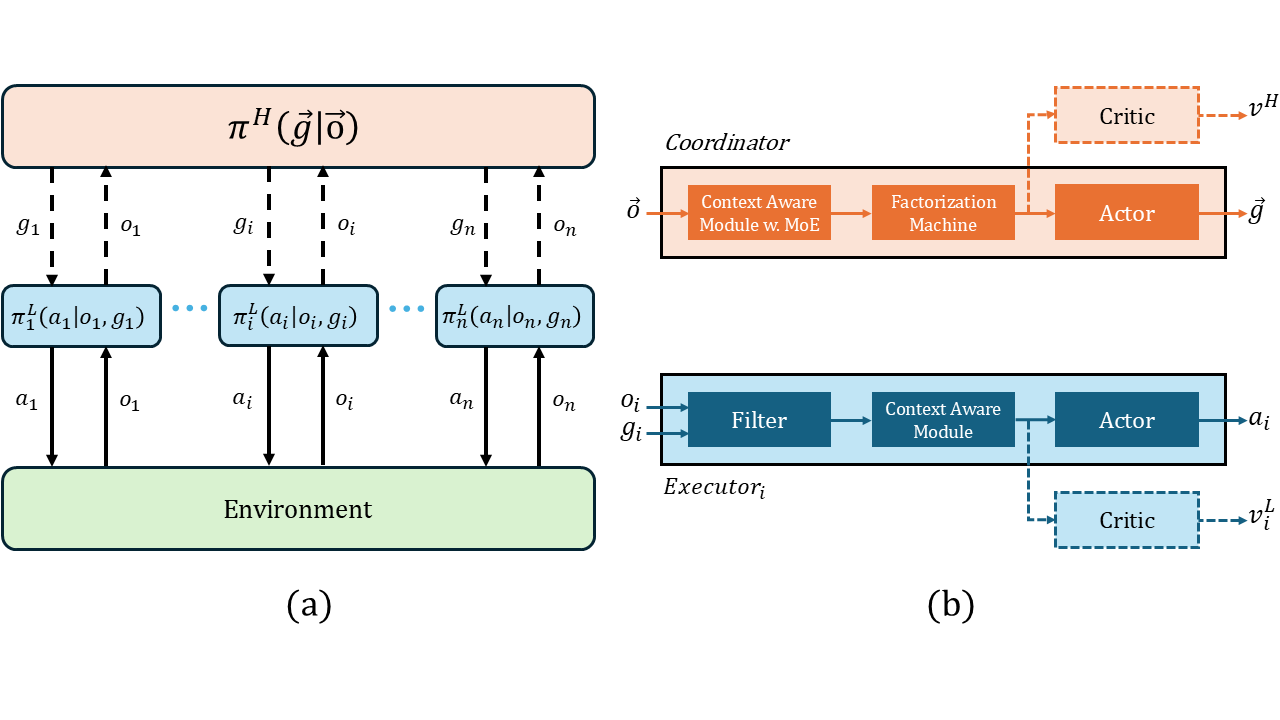
\includegraphics[width=\linewidth]{graphics/MoE.png}
%     \caption{An overview of the HiT-MAC framework. 
%     Figure 1(a) shows the two-level hierarchy of HiT-MAC. Periodically (every $k$ steps), the high-level policy (coordinator) $\pi^H(\overset{\rightarrow}{g}| \overset{\rightarrow}{o})$ collects joint observations $\overset{\rightarrow}{o} = (o_1, \dots, o_n)$ from sensors and distributes target-specific goals $g_i$ to each low-level policy (executor). The executor $\pi_i^L(a_i| o_i, g_i)$ then directly interacts with the environment to track its assigned targets. Figure 1(b) presents the details of the coordinator and executor. The critics for both are employed only during the training of the networks. The solid line represents actions taken at each step, while the dashed line indicates actions executed every $k$ steps.}
%     \label{fig:hs-flowchart}
%     
% \end{figure}

Both the coordinator and executors can be trained using contemporary single-agent reinforcement learning techniques (e.g., A3C) to optimize the expected future team reward (for the coordinator) and goal-specific rewards (for the executors). The team reward is influenced by the coverage rate, while the goal-conditioned reward reflects the performance of a sensor in tracking the assigned targets, assessed by the relative angle between the sensor and target. This dynamic can also be viewed as a collaborative effort between the coordinator and executors.

%In recent , the term \gls{iot} has attracted much attention from the world in general and the technology community in particular. One of the essential components of \gls{iot} is \gls{wsn}. Devices need to be equipped with sensor chips to detect phenomena in the physical environment and convert them into data on the Internet for users to process and analyze \cite{prasad2023energy,gong2023application}. Therefore, \glspl{wsn} are a significant contributor to the success of \gls{iot} \cite{jamshed2022challenges}. Sensors in the network collect data from a specific area and transmit monitoring data to a base station. Then, processing units generate reports to provide meaningful information to users.

%\glspl{wsn} are applied in various fields: military, healthcare, environment, agriculture, industry, transportation, etc. \cite{subramani2023multi, ijemaru2022wireless}. For example, sensors can be embedded in the body, on the skin, or on parts of clothing to monitor health status and measure health parameters such as blood pressure, heart rate, blood oxygen level, body temperature, and blood sugar of individuals, thereby enabling appropriate and timely patient treatment. Furthermore, \glspl{wsn} are used to monitor the environment in healthcare facilities for factors like temperature, humidity, light, dust, toxic gases, noise, etc. It helps maintain a safe and comfortable working environment and provides optimal treatment for patients.

%\glspl{wsn} are applied in almost every field, in various environments, and under different conditions. Therefore, sensor nodes are increasingly designed to be simple and lightweight for easy system integration. This leads to sensor nodes having limitations in computing power, energy, etc., as they need to collect and send data to the central hub for processing and analysis. Due to the values provided by \glspl{wsn}, there is an increasing number of research studies and significant scientific works published to address challenges in sensor networks, such as network lifespan, coverage capacity, connectivity, fault tolerance, load balancing, and security. This paper focuses on addressing the coverage challenge in \glspl{wsn}.

%Coverage issues can be divided into three different types: target coverage, area coverage, and barrier coverage. In this study, the authors are interested in solving the area coverage problem. When discussing the area coverage problem in \glspl{wsn}, one immediately thinks of monitoring the entire sensor placement area. This can be considered an extension of the target coverage problem, where every point in the monitored area is considered an object to be covered. The area coverage problem is divided into several sub-problems depending on criteria such as $100\%$ area coverage with minimized number of sensors, maximum area coverage with a given number of sensors, maximum area coverage with the minimum number of deployed sensor nodes, etc. Additionally, each problem can be further divided into various sub-problems by adding different criteria such as homogeneous sensors (sensors of the same type), heterogeneous sensors (different types of sensors), static sensors, dynamic sensors, and different sensor coverage models (binary model, probability model, ratio model, etc.). When adding different criteria to each problem, the network deployment also varies. However, in each problem studied above, many issues still need to be improved to reduce costs and increase stability in network deployment. Therefore, this paper focuses on researching the problem of maximum area coverage and minimum number of deployed nodes with heterogeneous sensors in \glspl{wsn}.

%The maximum area coverage and minimum number of deployed nodes problem with heterogeneous sensors in \glspl{wsn} has been proven to be an NP-hard problem \cite{yoon2013}, meaning that there is no polynomial-time algorithm to solve it, unless P=NP. Therefore, this paper approaches it using an approximation method with a meta-heuristic algorithm to solve the problem. The proposed algorithm is implemented and evaluated compared to previous studies and tested on synthetic data \cite{Al-Fuhaidi2020} and real-world datasets. Thus, researching this problem is scientifically and practically significant. In the next section, we present related studies on this issue.


%\subsection{Related work}

% \Glspl{hewsn} is implemented in many different types of problems. \citeauthor{Khedr2018} \cite{Khedr2018} sought to provide a coverage hole detection and recovery scheme. They proposed a three-phase scheme consisting of initialization, hole detection, and hole recovery phases. Each node acquired information about its neighboring nodes and determined whether it belonged to a hole. If that was the case, it entered the whole recovery phase with one of the two recovery modes: pro-active and re-active. \citeauthor{Bhat2020} \cite{Bhat2020} investigated a localization issue in \glspl{wsn}, which was used to identify the current location of the sensor nodes. They presented a range-free localization method called Harris Hawks optimization-based localization with area minimization. In \cite{Osamy2018} and \cite{Maurya2019}, the problems handling network lifetime maximization were considered. In particular, \citeauthor{Osamy2018} \cite{Osamy2018} attempted to maintain the maximal coverage and extend the network lifetime. Each node collected the necessary information about its sensing neighbors in the first phase. In the second phase, nodes with an energy level dropping below a specific threshold would be replaced. \citeauthor{Maurya2019} \cite{Maurya2019} aimed to maximize the energy efficiency of sensor nodes and proposed the so-called delay aware energy efficient, reliable routing technique. The three types of sensor nodes, named class-A, class-B, and class-C, were used in ascending order regarding the energy level, sensing range, and communication range. The idea was to assign each node to one of the following categories: agent node (AN), normal node (NN), candidate node (CN), or ring node (RN). In particular, NN and CN got the information of their nearest AN's position from RN and performed data aggregation to minimize unnecessary packets. After that, AN again performed data aggregation to minimize packet collision and then sent the data packet to sink. Nevertheless, the aforementioned research has failed to address the problems related to the coverage optimization of \glspl{hewsn}.
% \Glspl{wsn} is implemented in many different types of problems. \citeauthor{Narayan2023} \cite{Narayan2023} proposes a Fuzzy-based Energy Efficient Routing Protocol (E-FEERP) for Wireless Sensor Networks (WSNs) to optimize data transmission from Sensor Nodes (SN) to the Base Station (BS). It utilizes Particle Swarm Optimization (PSO) for cluster formation and incorporates a fuzzy logic approach based on average distance from BS, node density, energy, and communication quality. The protocol employs parallel fitness function computing to converge quickly to the optimal solution with fewer iterations. Inspired by bird flocking behavior, the PSO-based clustering algorithm enhances coverage and reduces computational overhead. \citeauthor{Vaiyapuri2022} \cite{Vaiyapuri2022} aimed to prolong network lifetime by proposing an IoT-enabled cluster-based routing (CBR) protocol for Information-Centric Wireless Sensor Networks (ICWSN), named CBR-ICWSN. The protocol employs a black widow optimization (BWO) based clustering technique to select optimal cluster heads (CHs) and utilizes an oppositional artificial bee colony (OABC) based routing process for path selection. \citeauthor{Trinh2022} \cite{Trinh2022} addresses energy consumption and congestion issues in wireless sensor networks (WSNs) by proposing a distributed fuzzy clustering scheme. The scheme utilizes two Fuzzy Logic Controllers (FLCs) to organize the WSN into clusters and select sink nodes. Multiple mobile sink nodes are considered, and cluster heads (CHs) use another FLC for fuzzy sink selection. CHs collaborate in multi-hop routing to minimize energy consumption. To address congestion, a distance-based version of the Random Early Detection (RED) congestion control method is proposed to intelligently drop data packets in forwarding nodes. Additionally, the effectiveness of the proposed FLCs is enhanced by tuning them using the Moth-Flame Optimization algorithm and minimizing their rules. \citeauthor{NJOYA2022212} \cite{NJOYA2022212} investigates a model for data aggregation in dense Wireless Sensor Networks (WSNs) with a single sink. The model divides the coverage region into patches and aggregates data at a single node in each patch before transmission. Nodes communicate only with others in the same sector. A linear programming problem is formulated to maximize system lifetime by minimizing maximum proportionate energy consumption. The optimal solution involves two transmission mechanisms: direct and stepwise. An exact formula for energy consumption rate is derived, with asymptotic forms agreeing with the linear programming solution. While the previous researches have fair contributions in optimizing data transmission, aggregation, congestion, energy consumption and network lifetime, they neglected \glspl{wsn} coverage, which is one of the most metrics determining the quality of a \gls{wsn}.

% Coverage optimization is one the very challenging problems presented in \glspl{wsn}, addressed in \cite{Zeng2023, Gou2023, Ammari2023, Wang2023, Cao2021}. \citeauthor{Zeng2023} \cite{Zeng2023} addressed the challenge of achieving adequate network coverage and connectivity in \glspl{hewsn} by proposing an improved wild horse optimizer algorithm (IWHO). The algorithm enhances population variety using SPM chaotic mapping during initialization, combines WHO with the Golden Sine Algorithm (Golden-SA) to improve accuracy and convergence speed, and incorporates opposition-based learning and the Cauchy variation strategy to escape local optima and expand the search space. \citeauthor{Gou2023} \cite{Gou2023} introduced VKECE-3D, an energy-efficient coverage enhancement method based on 3D-Voronoi partitioning and the K-means algorithm. It minimizes active nodes while ensuring coverage by deploying nodes randomly and then using a polynomial mutation strategy to enhance uniformity. Optimal perceptual radius is determined using the K-means algorithm and 3D-Voronoi partitioning, and a multi-hop communication and polling mechanism reduces energy consumption and extends network lifetime. \citeauthor{Ammari2023} \cite{Ammari2023} addressed the challenging k-coverage problem in planar \glspl{wsn}, aiming to ensure each point in the field is covered by at least k sensors simultaneously. It introduces several key contributions, including the identification of an optimal planar convex tile to maximize sensor usage, the proposal of sensor placement strategies based on desired coverage degree k with computed sensor densities, the introduction of a generalized approach using irregular hexagons (IRH(r/n)) and proof of their capability to tile the Euclidean plane, and the calculation of the relationship between sensor sensing range (r) and communication range (R) for the proposed strategies. \citeauthor{Wang2023} \cite{Wang2023} introduced a novel self-adaptive multi-strategy artificial bee colony (SaMABC) algorithm. It features a customized strategy pool and a finely-tuned adaptive selection mechanism tailored to the coverage optimization problem. Additionally, the algorithm is enhanced through the integration of a simulated annealing approach and dynamic search step to improve its ability to escape local optima. \citeauthor{Cao2021} \cite{Cao2021} presented an optimal coverage method for \glspl{hewsn} using an improved Social Spider Optimization (SSO) algorithm. The method aims to address coverage blind areas and redundancy caused by random sensor node deployment. It establishes a mathematical model for \gls{hewsn} coverage and utilizes a chaotic initialization method to enhance the global convergence speed. The SSO algorithm is improved by enhancing neighborhood and global search, as well as the matching radius. \citeauthor{deghbouch2022improved} \cite{deghbouch2022improved} introduced a novel sensor deployment scheme based on the improved bees algorithm (IBA) to optimize area coverage in both homogeneous and heterogeneous wireless sensor networks (WSNs). Incorporating a neighborhood shrinking procedure to enhance local search efficiency and a site abandonment procedure to prevent entrapment in local optima, the IBA yields superior results compared to two other metaheuristics: MCHSA \cite{panag2019maximal} and IFPA \cite{wang2019wireless}. It can be seen that the aforementioned works have taken into account network coverage as an essential aspect of the problems; however, the tackled problems are single-objective, which, in many cases, are simplifications and do not reflect the essence and characteristics of real-world problems.

% For a better representation of real-world challenges, some other researches attempted to solve the problems in \glspl{wsn} with multiple objectives \cite{Wang2022, Chen2023, Tam2021, Mazloomi2022, Hao2020}. \citeauthor{Wang2022} \cite{Wang2022} addressed the multi-objective problem of deploying wireless sensor networks with cooperative distance-based sensing coverage. The problem involves deploying sensor nodes to cover multiple target points within a deployment area, considering inner and outer coverage radii. Sensing coverages are categorized as full, no, or partial coverage based on distance. Additionally, cooperative sensing coverage is considered, where a target point may be covered by more than one sensor node. The objective is to select sensor nodes to maximize collective sensing coverage of all target points while minimizing total distances. The paper formulates this as a multi-objective optimization model and develops a solution procedure to find the best non-dominated solution set. In \cite{Chen2023}, \citeauthor{Chen2023} proposed an optimal deployment method for practical \glspl{hewsn} that balances reliability and deployment cost. The method aims to maximize coverage and connection degrees while minimizing overall deployment cost, considering differentiated sensing ranges and deployment costs of sensor nodes (SNs) in three-dimensional scenarios. This multi-objective optimization problem is non-convex, multimodal, and NP-hard. To address it, the authors introduce a novel swarm-based multi-objective optimization algorithm called the Competitive Multi-Objective Marine Predators Algorithm (CMOMPA). \citeauthor{Tam2021} \cite{Tam2021} addressed the critical issue of managing energy consumption in \glspl{wsn} to prolong network lifetime, considering the limited resources and computing capability of sensor nodes. Specifically, it focuses on optimizing network lifetime and the number of relay nodes in three-dimensional terrains. The proposed MOEA/D-LS algorithm aims to achieve a better tradeoff between these objectives by hybridizing a multiobjective evolutionary algorithm based on decomposition with a special local search to optimize its subproblems. By doing so, the algorithm offers a novel approach to effectively extend the network lifetime while considering the limited number of relay nodes, which is often overlooked in existing approaches. \citeauthor{Hao2020} \cite{Hao2020} focused on resource allocation in Multi-Radio Multi-Channel (MRMC) \glspl{wsn} to address energy consumption and Quality of Service (QoS) issues. It proposes a two-stage optimization algorithm that considers time slot assignment and then jointly optimizes power control and channel allocation. The algorithm aims to balance energy efficiency and network capacity while addressing constraints like link interference and load balance. It employs a graph coloring algorithm for conflict-free transmission and Multi-objective Hybrid Particle Swarm Optimization to obtain Pareto optimal solutions. \citeauthor{Mazloomi2022} \cite{Mazloomi2022} proposed MSOG, a novel method combining support vector regression and genetic algorithms, to model and optimize WSN indicators such as delay, received signal strength, packet arrival time, and successful packet delivery. By efficiently modeling and optimizing these indicators, MSOG aims to enhance WSN performance and reduce energy consumption. As observed, the researches mentioned above generally consider the homogeneous \gls{wsn} model instead of the heterogeneous model, making it less flexible to adapt to real-life situations and setups. Moreover, in those researches, the requirement (degree) of coverage and/or the availability of resources (in terms of quantity) are fixed instead of being considered an optimization objective. In \cite{Al-Fuhaidi2020}, \citeauthor{Al-Fuhaidi2020} aimed at maximizing the area coverage/target coverage of \glspl{hewsn}. The authors approached the area coverage problem as a point coverage problem by dividing the coverage area into rectangular cells, in which each cell's center served as a target. Aiming to balance network coverage and cost, \gls{hs} was proposed, which proved to achieve maximum coverage with fewer sensors compared to homogeneous deployment.

% In \cite{Al-Fuhaidi2020, NTHanh2019, HTTBinh2020, deghbouch2022improved}, the authors aimed at maximizing the area coverage/target coverage of \glspl{hewsn}. Specifically, \citeauthor{Al-Fuhaidi2020} \cite{Al-Fuhaidi2020} approached the area coverage problem as a point coverage problem and proposed \gls{hs}. The \gls{aoi} was divided into rectangular cells, and each cell center served as a target. In \gls{hs}, each harmony in the \gls{hm} corresponded to a potential solution to the optimization problem. Initially, the \gls{hm} was randomly generated. Then in each iteration, a new harmony was accepted if it was better than the worst one in the memory. Alternatively speaking, the \gls{hm} was updated. The objective function was evaluated based on the coverage ratio ($C_{\mathrm{ratio}}$), the HeWSN cost, and the minimum distance (MD). Specifically, a possible set of sensing ranges were testified to compute the MD. Since there are two sensing range types, the related time complexity was in the order of $\mathcal{O}(2^n)$, in which $n$ was the number of sensor nodes. Apart from this, \citeauthor{NTHanh2019} \cite{NTHanh2019} aimed to find the locations of sensors in order that the coverage area within the surveillance area was maximized by using a fixed number of sensors and sensing radii. The authors proposed a genetic algorithm where the population was initialized heuristically. In particular, sensors were gradually deployed, one at a time, to form an individual. The fitness function was then calculated as the area covered inside the surveillance area through an integral method. \citeauthor{HTTBinh2020} \cite{HTTBinh2020} inspected a problem similar to \cite{NTHanh2019} but in a vast extension by taking into account the presence of obstacles in the surveillance area. Two algorithms were proposed by exploiting the genetic algorithm and particle swarm optimization. For the genetic algorithm, the population was first initialized by the three different mechanisms consisting of the random, heuristic, and new heuristic. The fitness function was then computed as a sum of the three different components: an overlap between the coverage areas of the sensors, an overlap between the coverage areas of the sensors and these obstacles, and a part of the coverage areas of the sensors that are out of the surveillance region. \citeauthor{deghbouch2022improved} \cite{deghbouch2022improved} proposed Improved Bee Algorithm (IBA) to tackle the target coverage problem in \glspl{hewsn} with binary disk coverage model and fixed number of each sensor type. In the paper, IBA is proved by experiments to have better results than two other metaheuristic approaches solving the same problem, which are MCHSA \cite{panag2019maximal} and IFPA \cite{wang2019wireless}.

%The area coverage problems have captured significant attention from researchers in one of the two types mentioned above: full coverage, which insists on monitoring the whole area, or partial coverage, which aims to maximize the coverage rate. Some researchers have addressed the full area coverage problem, such as in \cite{Ammari2023}, \citeauthor{Ammari2023} addressed the challenging k-coverage problem in planar \glspl{wsn}, aiming to ensure each point in the field is covered by at least k sensors simultaneously while trying to minimize sensor density. Their contributions include an optimal planar convex tile to maximize sensor usage, several sensor placement strategies based on the coverage degree k, a generalized approach using irregular hexagons (IRH(r/n)) and proof of their capability to tile the Euclidean plane.

%However, a large part of the contemporary works in the literature focus on maximizing (partial) coverage using a fixed number of resources.
%\citeauthor{Zeng2023} \cite{Zeng2023} addressed the challenge of achieving adequate network coverage and connectivity in \glspl{hewsn} by proposing an improved wild horse optimizer algorithm (IWHO). The algorithm enhances population variety using SPM chaotic mapping, combines WHO with the Golden Sine Algorithm (Golden-SA) to improve accuracy and convergence speed, and incorporates opposition-based learning and the Cauchy variation strategy to escape local optima and expand the search space.
%\citeauthor{Wang2023} \cite{Wang2023} introduced a novel self-adaptive multi-strategy artificial bee colony (SaMABC) algorithm. It features a customized strategy pool and a finely tuned adaptive selection mechanism tailored to the coverage optimization problem. Additionally, the algorithm is enhanced by integrating of a simulated annealing approach and dynamic search step to improve its ability to escape local optima.
%\citeauthor{HTTBinh2020} \cite{HTTBinh2020} tackled the challenge of maximizing coverage in \gls{hewsn} with obstacles in the area. The authors proposed Genetic Algorithm and Particle Swarm Optimization. The contributions include heuristic initialization, a new fitness function, modified virtual force algorithm, and adjustments to the calculation of inertia weight and sub-population head individuals' influence.
%\citeauthor{deghbouch2022improved} \cite{deghbouch2022improved} introduced a novel sensor deployment scheme based on the improved bees algorithm (IBA) to optimize area coverage in both homogeneous and heterogeneous \glspl{wsn}. The method incorporated a neighborhood shrinking procedure to enhance local search efficiency and a site abandonment procedure to prevent entrapment in local optima.

%The works above have taken into account network coverage as an essential aspect of the problems; however, the tackled problems are single-objective, which, in many cases, are simplifications and do not reflect the essence and characteristics of real-world issues. Having acknowledged that, some other researchers attempted to solve the problems in \glspl{wsn} with multiple objectives.

%\citeauthor{Cao2021} \cite{Cao2021} addressed the issue of relocating deployed sensors which seeks to maximize area coverage and network lifetime in \glspl{hewsn}. The network model involves the loss of mobile sensor energy during movement. They proposed an improved Social Spider Optimization (SSO) algorithm, which addresses coverage blind areas and redundancy caused by random sensor node deployment. It employs a chaotic initialization method to enhance the global convergence speed.
%\citeauthor{Gou2023} \cite{Gou2023} dealt with a problem similar to \cite{Cao2021} but in three-dimensional spaces. They introduced VKECE-3D, a method based on 3D-Voronoi partitioning and the K-means algorithm. A polynomial mutation strategy is used to enhance the uniformity of the nodes. Optimal perceptual radius is determined using the K-means algorithm and 3D-Voronoi partitioning. Finally, a multi-hop communication and polling mechanism reduces energy consumption.

%In \cite{Wang2022} and \cite{Chen2023}, the \gls{wsn} model predefines the set of candidate locations for sensors to be deployed.
%\citeauthor{Wang2022} \cite{Wang2022} addressed the problem of deploying sensors with distance-based sensing coverage. The problem involves deploying sensor nodes to cover the targets with coverage degree of k (k-coverage). Sensing coverages are categorized as full, no, or partial coverage based on distance. The objective is to select sensor nodes to maximize collective sensing coverage of all target points while minimizing total distances between targets and sensors.
%\citeauthor{Chen2023} \cite{Chen2023} proposed an optimal deployment method for \glspl{hewsn} that balances reliability and deployment cost. The method aims to maximize coverage and connection degrees while minimizing overall deployment cost, considering differentiated sensing ranges and deployment costs of sensor nodes in three-dimensional scenarios. To address it, the authors introduce a novel swarm-based optimization based on Marine Predators Algorithm (MPA).

%Some other papers sought to minimize the number of nodes as one of the objectives. \citeauthor{Tam2021} \cite{Tam2021} focused on optimizing network lifetime and the number of relay nodes in three-dimensional terrains. The proposed MOEA/D-LS algorithm aims to achieve a better tradeoff between these objectives by hybridizing an evolutionary algorithm based on decomposition with a special local search.

%There are not many works addressing the multi-objective problem of maximizing area coverage and minimizing the number of nodes in \glspl{hewsn}. \citeauthor{Al-Fuhaidi2020} \cite{Al-Fuhaidi2020} proposed a method to solve such a problem by dividing the area of interest into equal cells and treating each cell as a target. They proposed \gls{hs}, in which each harmony in the \gls{hm} corresponded to a potential solution to the problem. Initially, the \gls{hm} is randomly generated. Then, in each iteration, a new harmony replaces the worst harmony in the memory if it is better. The objective function was evaluated based on the coverage ratio ($C_{\mathrm{ratio}}$), the deployment cost, and the minimum distance ($MD$) between sensors. \citeauthor{Sharma2019Modeling3W} \cite{Sharma2019Modeling3W} solves the same multi-objective problem with binary disk coverage model in 3D space using \gls{hs} scheme. They proposed an objective function that is similar to \cite{Al-Fuhaidi2020}, only differing in some coefficients.  

% Some works addressed different problems of coverage in \glspl{wsn}. \citeauthor{cao2018deployment} \cite{cao2018deployment} addressed the deployment problem of \glspl{wsn} in complex 3D industrial spaces with obstacles. It focused on maximizing coverage using heterogeneous directional sensor nodes and prolonging network lifetime with relay nodes. A modified 3D coverage model and a lifetime model with reliability constraints were introduced for mathematical analysis. Two particle swarm optimization methods, CCPSO2 and CLPSO, were employed. \citeauthor{zaimen2020overview} \cite{zaimen2020overview} explored optimizing \glspl{wsn} deployment in smart buildings, emphasizing the integration of IoT to enhance data accuracy, reduce energy consumption, and ensure user comfort. It highlighted the challenge of positioning sensor nodes in environments with heterogeneous obstacles to achieve full coverage and connectivity. After reviewing various solutions, the paper proposed a novel approach using Building Information Modeling (BIM) to obtain real-time data for optimizing sensor deployment. \citeauthor{saad2020toward} \cite{saad2020toward} addressed the deployment of \glspl{wsn} in realistic 3D environments. It introduced a Bresenham line-of-sight based coverage model to accurately reflect the behavior of sensors and the environment. The deployment problem was reformulated mathematically and solved using an enhanced multi-objective genetic algorithm, RASP, featuring adaptive and guided genetic operators. Performance improvements are achieved through search space reduction and sampling-based evaluation.

%Some works addressed various coverage problems in \glspl{wsn}. \citeauthor{cao2018deployment} \cite{cao2018deployment} focused on deploying \glspl{wsn} in complex 3D industrial spaces with obstacles, using heterogeneous directional sensors and relay nodes to maximize coverage and prolong network life, employing two particle swarm optimization methods. \citeauthor{zaimen2020overview} \cite{zaimen2020overview} optimized \glspl{wsn} deployment in smart buildings by integrating IoT for better data accuracy, reduced energy consumption, and user comfort, using BIM for real-time data to optimize sensor placement. \citeauthor{saad2020toward} \cite{saad2020toward} tackled WSN deployment in realistic 3D environments with a Bresenham line-of-sight coverage model and an enhanced multi-objective genetic algorithm for improved performance.

%While there have been several attempts at optimizing area coverage in \glspl{hewsn}, we observe that the authors in \cite{Ammari2023,Zeng2023,Wang2023,HTTBinh2020,deghbouch2022improved} only solved single-objective problems, which aim at maximizing area coverage itself, with other factors being predetermined, such as the number of nodes. Such approaches lack flexibility in real-life scenarios, where the number of network resources or configurations thereof may vary over time according to different needs. Besides, the authors in \cite{Zeng2023,Cao2021,HTTBinh2020,deghbouch2022improved} only considered the binary disk coverage model, which is simple and does not reflect the way sensors work in real life. Moreover, the method in \cite{Al-Fuhaidi2020} faces several disadvantages, such as falling into local optimum due to random initialization, a high computational time (exponential time complexity), and the fitness function not doing a good job of representing the quality of a solution, not to mention that its performance on large-scale area is very uninspiring. As a result, in this paper, we propose changes to different disadvantageous components of the \gls{hs} algorithm proposed in \cite{Al-Fuhaidi2020}. In addition, we construct a real-world dataset to evaluate the efficiency of the proposals. We strongly believe our work will help improve the quality of solutions and running time in various datasets.

%\subsection{Motivations and Contributions}

% Coverage is a fundamental issue concerning \glspl{wsn}. Nonetheless, a high proportion of research about coverage considers the homogeneous sensor model, where sensors have the same hardware specifications, such as sensing range, computational capability, and energy level. This is an oversimplified model and not common in real life as sensors tend to be heterogeneous or deliberately designed so due to numerous reasons \cite{Cao2021}. For example, a cluster head is often a high-end node with more powerful computational performance and battery capacity compared to other low-end nodes. Moreover, \glspl{hewsn} is said to be able to achieve a better balance between performance and cost of deploying compared to homogeneous \gls{wsn} \cite{Wang2013}. Consequently, in this research, we investigate the problem of maximizing area coverage in a \gls{hewsn}.

%Coverage is a fundamental issue concerning \glspl{wsn}. Nonetheless, a high proportion of research about coverage considers the homogeneous sensor model, where sensors have the same hardware specifications, which is oversimplified and sometimes deliberately designed so due to numerous reasons \cite{Cao2021}. Moreover, \glspl{hewsn} are said to achieve a better balance between performance and cost of deploying compared to homogeneous \glspl{wsn} \cite{Wang2013}. Consequently, in this research, we investigate the problem of maximizing area coverage in a \gls{hewsn}. In terms of this problem, there are few works (\cite{Al-Fuhaidi2020}, \cite{deghbouch2022improved}) which need more extensive experiments on large-scale environments or realistic datasets. Those works only consider the problem in a 2D environment, which is not feasible in real-case scenarios. Therefore, our work is the first to solve the area coverage problem with heterogeneous sensors in a 3D area. Moreover, the adaptation of \gls{hs} in existing work \cite{Al-Fuhaidi2020} solving the problem is simple, which may bring poor performance in complex and large-scale areas, raising the need for a more dedicated adaptation of \gls{hs}. Hence, we enhance the efficiency of \gls{hs} applied for the coverage problem in \glspl{wsn}, stepping toward a better solution.

% Since the optimization problems of node deployment in \glspl{wsn} are inherently non-convex, \gls{hs} will not provide the optimum solution if population initialization is not executed properly, resulting in a local optimum only. In this paper, we enhance the efficiency of \gls{hs} applied for the coverage problem in \glspl{wsn}, stepping toward a better solution. 

Our main contributions are listed as follows:
%\begin{itemize}
 %   \item We formulate a multi-objective problem finding the locations of the sensor nodes with the objectives of maximizing coverage and minimizing the number of sensors. This is a non-convex optimization problem with a discrete feasible domain.
  %  \item We propose four enhancements for the \gls{hs} algorithm for solving the problem, which include a novel initialization strategy to avoid a bad sub-optimal solution for large-scale \glspl{wsn}, which occurs due to the complicated network nature with many discrete optimization variables; an innovative sampling strategy to significantly reduce time complexity without heavily affecting the solution efficiency; a weighted fitness function; and different new component-integrated fitness functions to achieve better metrics evaluation. We also extend our solution to 3D environments to adapt to real-case scenarios.
   % \item We provide a dataset of real-life terrains for experiments with 3D environments. The dataset consists of four provinces in Vietnam, which are Bac Giang, Son La, Ha Noi, and Thai Binh.
    
  %  \item We conduct in-depth experiment analysis to effectively evaluate the quality of our enhancement proposals and compare them with the baseline methods on both 2D areas and our proposed 3D dataset.
    % \item We propose a algorithm that yields a good sub-optimal solution to the coverage maximization problem by exploiting \gls{hs}. The proposed algorithm involves a number of hyperparameters, thereby providing the flexibility to find and improve the solution.
    % \item We suggest different initialization strategies to avoid a bad sub-optimal solution for large-scale \glspl{wsn}, which occurs due to the complicated network nature  with many discrete optimization variables.
    % \item We present the different methods to calculate the fitness function adapted to different measurement metrics, which are used for evaluating the solution's efficiency, and therefore improving the flexibility of the solution.
%\end{itemize}

% 
% \subsection{Paper Outline and Notations}
% 
%The rest of this paper is organized as follows. Section~\ref{Sec:HeWSN} introduces the \gls{hewsn} deployment model, the coverage, connection, and energy model. Sections~\ref{sec:formulate} and \ref{sec:app} provide problem formulation and its applications, respectively. Section~\ref{Sec:ProposedMethods} presents \gls{hs} in detail and proposes several strategies to improve its efficiency. Section~\ref{sec:3d_extension} presents the extension of the problem and the solutions to 3D environments. Meanwhile, Section~\ref{Sec:ExpRe} presents various experiment scenarios and the corresponding results. Finally, Section~\ref{Sec:Conclusion} draws the main conclusions. All of the notations used in this paper are provided in Table~\ref{tab:notations}.

% \begin{table}
% % \vspace{-4cm}
%     \caption{Table of notations.}
%     \label{tab:notations}
%     \centering
%     % { \footnotesize
%     \begin{tabular}{|cp{25em}|} \hline
%         \textbf{Notation} & \multicolumn{1}{c|}{\textbf{Definition}} \\ \hline
%         $rand((a, b))$ & a random number in the interval $(a, b)$. The same applies for $[a, b)$, $(a, b]$ and $[a, b]$. \\ \hline
%         $randint(a, b)$ & a random integer $\geq a$ and $\leq b$ \\ \hline
%         $w_{cell}$ & cell width \\ \hline
%         $h_{cell}$ & cell height \\ \hline
%         $n_{cell}$ & number of cells \\ \hline
%         $X^{(L)}_i$ & $x$ lower bound of sensor type $i$ \\ \hline
%         $Y^{(L)}_i$ & $y$ lower bound of sensor type $i$ \\ \hline
%         $X^{(U)}_i$ & $x$ upper bound of sensor type $i$ \\ \hline
%         $Y^{(U)}_i$ & $y$ upper bound of sensor type $i$ \\ \hline
%         $x^{(L)}_s$ & $x$ lower bound of sensor $s$ \\ \hline
%         $y^{(L)}_s$ & $y$ lower bound of sensor $s$ \\ \hline
%         $x^{(U)}_s$ & $x$ upper bound of sensor $s$ \\ \hline
%         $y^{(U)}_s$ & $y$ upper bound of sensor $s$ \\ \hline
%         $x_s$ & $x$-coordinate of sensor (target, etc.) $s$ \\ \hline
%         $y_s$ & $y$-coordinate of sensor (target, etc.) $s$ \\ \hline
%         $S$ & set of sensors \\ \hline
%         $S_i$ & set of type $i$ sensors ($i = 1, 2$) \\ \hline
%         $R_i$ & sensing range of type $i$ sensor ($i = 1, 2$) \\ \hline
%         $r_s$ & sensing range of sensor $s$ \\ \hline
%         $R^{(u)}_i$ & uncertain sensing range of type $i$ sensor ($i = 1, 2$) \\ \hline
%         $r^{(u)}_s$ & uncertain sensing range of sensor $s$ \\ \hline
%         $d(A, B)$ & Euclidean distance between point $A$ and $B$ \\ \hline
%         $P(t, s)$ & probability of target $t$ being covered by sensor $s$ \\ \hline
%         $P(t)$ & probability of target $t$ being covered by at least one sensor \\ \hline
%         $TH_{cov}$ & acceptable coverage threshold \\ \hline
%     \end{tabular}%}
% \end{table}


\section{Preliminaries} \label{Sec:HeWSN}
\noindent\textbf{Problem Definition.} The target coverage problem considers how to use a number of active sensors
to continuously cover maximum number of targets. In this case, there are n sensors and m mobile
targets in the environment. Sensors are randomly placed in the environment with limited coverage
range. The targets randomly walk around the environment. A target is covered by the sensor network,
once it is monitored by at least one sensor. The orientation of the sensor is adjustable, but the
changing angle at each step is restricted considering the physical constraints. Besides, considering
the efficiency problem, every movement will take additional cost in power.

\noindent\textbf{Dec-POMDPs.} The target coverage issue in sensor networks can be effectively modeled as a Decentralized Partially Observable Markov Decision Process, which is described by the tuple \( \langle N, S, \{A_i\}_{i \in N}, \{O_i\}_{i \in N}, R, P_r, Z \rangle \), where \( N \) represents a group of \( n \) agents, identified as \( \{1, 2, \dots, n\} \). The set \( S \) includes all possible states of the environment, while each agent \( i \) has a set of available actions \( A_i \), which together form joint actions \( \overset{\rightarrow}{a_t} = (a_{1,t}, \dots, a_{n,t}) \). \( O_i \) denotes the observation space for agent \( i \), and its local observation \( o_{i,t} \) comes from the observation function \( Z(o_{i,t}\mid s_t, \overset{\rightarrow}{a_t}) \). The reward function \( R \) assigns a shared reward to the team based on the state, and \( P_r \) defines the probabilities for transitioning between states based on joint actions.
At each time step \( t \), agents observe \( o_{i,t} \) and choose an action \( a_{i,t} \) according to their individual policy \( \pi_i(a_{i,t} \mid o_{i,t}) \). The joint action \( \overset{\rightarrow}{a_t} \) then causes a transition from state \( s_t \) to \( s_{t+1} \) as dictated by \( P_r(s_{t+1} \mid s_t, \overset{\rightarrow}{a_t}) \). As the process continues, each agent receives a new observation \( o_{i,t+1} \), and the team is rewarded with \( r_{t+1} = R(s_{t+1}) \). In this cooperative setup, the goal is to optimize the group policy \( \langle \pi_1, \dots, \pi_n \rangle \) to maximize the total expected reward over time, using a discount factor \( \gamma \) and planning horizon \( T \), represented as \( E_{\overset{\rightarrow}{a_t} \sim \langle \pi_1, \dots, \pi_n \rangle} \left[ \sum_{t=1}^{T} \gamma^t r_t \right] \) 

% \vspace{1em}

\noindent\textbf{Hierarchical MMDPs.} The coverage problem is structured into two layers: high-level coordination and low-level execution. The high-level agent, acting as a coordinator, manages \( n \) low-level agents (executors) over time to maximize the total team reward \( \sum_{t=1}^{T} \gamma^t r_t \). The coordinator's policy \( \pi_H(\mathbf{g}_t \mid \mathbf{o}_t) \) assigns goals \( \mathbf{g}_t = (g_{0,t}, g_{1,t}, \dots, g_{n,t}) \) to the executors based on their combined observations \( \mathbf{o}_t \), which are collected from the executors. Once executor \( i \) receives a goal \( g_{i,t} \) at time step \( t \), it works locally to fulfill that goal over \( k \) steps, aiming to maximize the cumulative goal-dependent reward \( r^L_{i,t} = R^L(s_t, g_{i,t}) \) by executing actions according to the policy \( \pi^L_i(a_{i,t} \mid o_{i,t}) \). Since the coordinator interacts with the executors at intervals of \( k > 1 \) steps, the high-level transitions can be modeled as a semi-Markov Decision Process (semi-MDP). Meanwhile, the executors operate in a decentralized fashion, akin to Dec-POMDPs, but their actions and rewards are guided by their assigned goals \( g_{i,t} \). This framework, combining the semi-MDP with Dec-POMDPs, creates a two-tier hierarchical system for multi-agent decision-making, referred to as hierarchical multi-agent MDPs (HMMDPs).

% \vspace{1em}

\noindent\textbf{Attention Modules.} Attention mechanisms have garnered significant interest due to their strong performance across various tasks. Moreover, the self-attention module is capable of processing inputs of varying sizes in a manner that is independent of their order. In this study, we utilize the scaled dot-product attention. Specifically, the output matrix \( H \) is calculated as a weighted sum of the values, expressed as:

\[
H = \text{Att}(Q, K, V) = \text{softmax}\left(\frac{QK^T}{\sqrt{d_k}}\right)V \quad 
\] where \( d_k \) represents the dimension of a key. The matrices \( K \), \( Q \), and \( V \) are derived from the input matrix \( X \) using parameter matrices \( W_q \), \( W_k \), and \( W_v \). These are computed as follows:

\[
Q = \tanh(W_qX), \quad K = \tanh(W_kX), \quad V = \tanh(W_vX) \quad 
\] The context feature \( C \) is obtained by summing the elements in \( H \) additively, where \( h_i \) denotes an individual element and \( N \) signifies the total number of elements in \( H \).

% \vspace{1em}
\noindent\textbf{Factorization Machine.} Factorization Machines (FM) are a versatile model designed to handle sparse, high-dimensional data, particularly in recommendation systems. FM models both linear and pairwise feature interactions, expressed as:

\[
\hat{y} = w_0 + \sum_{i=1}^{n} w_i x_i + \sum_{i=1}^{n} \sum_{j=i+1}^{n} \langle v_i, v_j \rangle x_i x_j
\] where $w_0$ is the global bias, $w_i$ represents feature weights, and $v_i$ is the latent vector associated with feature $i$. This formulation allows FMs to efficiently capture interactions between features without explicitly defining them, making it suitable for tasks like collaborative filtering, regression, and classification. FMs require fewer parameters compared to traditional interaction models, which helps in managing data sparsity effectively. This adaptability allows FMs to excel in a variety of machine learning applications, especially in scenarios involving high-dimensional inputs.

% \vspace{1em}
\noindent\textbf{Mixture of Experts.} The Mixture of Experts (MoE) framework addresses complex tasks by utilizing a set of specialized sub-models, known as experts, each focusing on distinct aspects of the data. The gating network $g$ dynamically selects the top $k$ experts to activate based on the input $x$. This selection is represented mathematically as:

\[
g_i(x) = 
\begin{cases} 
\frac{ef_i(x)}{\sum_{j=1}^{N} ef_j(x)} & \text{if } i \in \text{Top } k \\ 
0 & \text{otherwise}
\end{cases}
\]where $f_i(x)$ is a scoring function that determines the relevance of expert $i$ for the input, and $\text{Top } k$ denotes the indices of the top $k$ experts based on their scores.
Each selected expert $E_i$ produces an output based on $x$:

\[
y_i = E_i(x)
\]The final output $y$ of the MoE model is computed as a weighted sum of the outputs from the selected experts:

\[
y = \sum_{i \in \text{Top } k} g_i(x) \cdot E_i(x)
\]This approach allows the model to focus its computational resources efficiently by engaging only the most relevant experts for each input. The training process involves jointly optimizing both the experts and the gating network, ensuring that the selection mechanism enhances the relevance of the activated experts. This hierarchical structure not only supports scalability but also improves overall model performance across various applications. Thus, the MoE framework offers a robust approach to multi-task learning, effectively leveraging the strengths of multiple specialized models while maintaining efficiency through selective activation.


%\quad The \gls{hewsn} deployment model and problem formulation are introduced in \cite{Al-Fuhaidi2020}. Hence, we will reintroduce those terms using our own denotations and symbols in order to be clearer and more appropriate for our paper. This section consists of three subsections.

%This section consists of three parts. The first part provides the specifications of the \gls{aoi} and sensor types. The second part introduces the \gls{hewsn} deployment model. Next, the third part presents the categorization of coverage based on the \gls{psm}. Finally, the fourth part presents the connection and energy model used in this paper.

% Finally, the fourth part formulates the coverage optimization problem.

%\subsection{\glsentryshort{aoi} and sensor specifications}


%In order to evaluate the system performance, we first provide the specifications of the \gls{aoi} and sensors, as follows:
%\begin{itemize}
    %\item \textit{\Gls{aoi} specifications}: The \gls{aoi} is a rectangle of width $W$~[\unit{\metre}] and height $H$~[\unit{\metre}], divided into various rectangular cells whose sizes depend on the sensors' sensing range. Without loss of generality, we assume that all cells have the same size of $w_{cell} \times h_{cell}$. Hence, the numbers of cells along the $Ox$ axis and $Oy$ axis are $\left\lceil \frac{W}{w_{cell}} \right\rceil$ and $\left\lceil \frac{H}{h_{cell}} \right\rceil$, respectively. Then, the total number of cells in the \gls{aoi} is:
    %\begin{equation}
       % n_{cell} = \left\lceil \frac{W}{w_{cell}} \right\rceil \times \left\lceil \frac{H}{h_{cell}} \right\rceil,
    %\end{equation}
    %where $\lceil \cdot \rceil$ is the ceiling function. We remodel the original area coverage problem into a target coverage problem. Particularly, each target is located at the center of a cell. We assume that the more targets are covered, the more efficiently we can deploy the \gls{wsn} inside the \gls{aoi}. 

    %\item \textit{Sensor specifications}: We consider two types of heterogeneous sensors in terms of sensing ranges: type 1 with sensing range $R_1$ and type 2 with sensing range $R_2$ ($R_1 > R_2$). This configuration can be applied in various use cases. For instance, in a smart home security system, sensors with different sensing ranges can be utilized. For instance, sensors with a small range can be placed in rooms or smaller areas, while sensors with a longer range can cover larger spaces like hallways or common areas. This combination ensures comprehensive coverage throughout the home. Another use case is that environmental monitoring applications often require sensor networks to collect data over a wide area. By deploying sensors with different sensing ranges, we can optimize coverage and resource allocation. Sensors with a small range can be deployed in densely populated areas, while sensors with a longer range cover larger open spaces. In addition, each type of sensor has an uncertain sensing range $R^{(u)}_i < R_i$. Besides, in this model, the sensors are stationary (i.e., they cannot move in the \gls{aoi}). Fig.~\ref{fig:AoI} illustrates the \gls{aoi} and heterogeneous sensors.
%\end{itemize}

%\begin{figure}
    % \centering
    % \includegraphics[width=0.6\linewidth]{graphics/AoI.pdf}
    % \caption{The \gls{aoi} divided into equal-sized cells and some deployed heterogeneous sensors. Each sensor establishes a one-hop connection to the base station (see Section \ref{sec:energy})}
    % \label{fig:AoI}
    
% \end{figure}

% \subsection{\glsentryshort{hewsn} initialization}

% In this part, we present the initialization scheme for \gls{hewsn}. First, each sensor location is represented by a coordinate $(x,y)$, where $x$ and $y$ are randomized in the \gls{aoi} range. However, we do not want a sensor to be too close to the boundaries of the \gls{aoi} because this would be a waste of sensing capability. Specifically, we do not want any part of the area inside the radius $(R-R^{(u)})$ from each sensor to be out of the AoI because, according to PSM \cite{Li2005}, every point in this area has $100\%$ coverage from the corresponding sensor.  Hence, the lower and upper bounds of $x$ and $y$ for each sensor type ($i = 1, 2$) are defined as follows:
% \begin{align}
%     X^{(L)}_i & = R_i - R^{(u)}_i, \\
%     Y^{(L)}_i & = R_i - R^{(u)}_i, \\
%     X^{(U)}_i & = W - (R_i - R^{(u)}_i), \\
%     Y^{(U)}_i & = H - (R_i - R^{(u)}_i).
% \end{align}

% As the initialization of sensors is random, the $x$-coordinate and $y$-coordinate of each sensor $s$ are randomized uniformly between their lower and upper bounds:
% \begin{align}
%     x_s & = x^{(L)}_s + (x^{(U)}_s - x^{(L)}_s) \times rand((0, 1)), \label{eq:xsLU} \\
%     y_s & = y^{(L)}_s + (y^{(U)}_s - y^{(L)}_s) \times rand((0, 1)). \label{eq:ysLU}
% \end{align}

% For example, if $s$ is of type 1, then $x^{(L)}_s = X^{(L)}_1$, and so on. We note that \eqref{eq:xsLU} and \eqref{eq:ysLU} ensure that $x$ and $y$ lie between the lower and upper bounds. However, we need to restrict the number of sensors generated as we do not want the number of sensors to be too low or too high. Specifically, along the $x$-axis, the distance between two consecutive sensors of type $i$ should not be larger than $2(R_i + R^{(u)}_i)$. Otherwise, a point with zero coverage will exist between the two corresponding circles. Additionally, along the $x$-axis, the distance between two consecutive sensors of type $i$ is not necessary to be smaller than $2(R_i - R^{(u)}_i)$ because with this distance, all the points between those two sensors already have $100\%$ coverage. The same logic is applied to $y$-axis. Hence, we define the minimum and maximum number of sensors as follows \cite{Alia2017}:
% \begin{align}
%     |S|_{min} & = \frac{W}{2(R_i + R^{(u)}_i)} \times \frac{H}{2(R_i + R^{(u)}_i)}, \label{eq:|S|min} \\
%     |S|_{max} & = \frac{W}{2(R_i - R^{(u)}_i)} \times \frac{H}{2(R_i - R^{(u)}_i)}. \label{eq:|S|max}
% \end{align}
% The denominators of \eqref{eq:|S|min} and \eqref{eq:|S|max} have a factor of $2$ to obtain the inner and outer diameters of the probable sensing range.

% \subsection{Categorization of coverage probability based on the \glsentryshort{psm}}

% There are two main sensing models used in \glspl{wsn}. The first is the Binary Sensing Model, which only considers the sensing range. A target is considered covered if it lies within the sensing range of a sensor and vice versa. Despite its simplicity, it cannot describe other elements that affect the sensors, such as signal reduction due to long distances or signal interference among sensors. Hence, we consider a \gls{psm} in this paper. The model provides various parameters to make the model more practical. At a certain point, the probability that a sensor covers a target decreases and finally reaches $0$ as the distance between them increases \cite{Li2005}, as formulated in \eqref{eq:PSM} and illustrated in Figure~\ref{fig:PSM}:
% \begin{multline}
%     P(t, s) = \begin{cases}
%         1 & \text{if } d(s, t) < r_s - r^{(u)}_s, \\
%         e^{\left( - {\frac{\alpha_1\lambda_1^{\beta_1}}{\lambda_2^{\beta_2}} + \alpha_2}\right)} & \text{if } r_s - r^{(u)}_s \leq d(s, t) < r_s + r^{(u)}_s, \\
%         0 & \text{otherwise } (r_s + r^{(u)}_s \leq d(s, t)).
%     \end{cases}
%     \label{eq:PSM}
% \end{multline}

% \begin{figure}
%     \centering
%     \includegraphics[width=0.6\linewidth]{graphics/PSM.pdf}
%     \caption{Illustration of \Gls{psm}.}
%     \label{fig:PSM}
    
% \end{figure}

% In \eqref{eq:PSM} and Figure~\ref{fig:psm-graph}, $P(t, s)$ denotes the probability that sensor $s$ covers target $t$, $d(s, t)$ represents the Euclidean distance between sensor $s$ and target $t$, which is given by:
% \begin{equation}
%     d(s, t) = \sqrt{(x_s - x_t)^2 + (y_s - y_t)^2}.
% \end{equation}
% Besides, we introduce four hyperparameters for the \gls{psm} which express the physical characteristics of the sensor: $\alpha_1, \alpha_2, \beta_1, \beta_2$. In this paper, we set $\alpha_1=-1, \alpha_2=0, \beta_1=1, \beta_2=0.5$ for every sensor type. Meanwhile, $\lambda_1$~[\unit{\metre}] and $\lambda_2$~[\unit{\metre}] are calculated as in \cite{Li2005}:
% \begin{align}
%     \lambda_1 = r^{(u)}_s - r_s + d(s, t), \\
%     \lambda_2 = r^{(u)}_s + r_s - d(s, t).
% \end{align}

% The graph of $P(t, s)$ with respect to $d(s, t)$ is shown in Fig.~\ref{fig:psm-graph}, given $r_s=\qty{10}{\metre}$ and $r^{(u)}_s=\qty{5}{\metre}$. We can see that $P(t, s)$ is a continuous and decreasing function with respect to $d(s, t)$ on $[0, \infty]$, which means the sensing ability of sensors decreases when the distance increases.

% \begin{figure}
%     \centering
%     \includegraphics[width=0.8\linewidth]{graphics/psm_graph.pdf}
%     \caption{The correlation between the probability that sensor $s$ covers target $t$ ($P(t, s)$) and their distance ($d(s, t)$).}
%     \label{fig:psm-graph}
    
% \end{figure}
% With respect to the network, the probability of $t$ being covered is \cite{Zou2003}:
% \begin{equation}
%     P(t) = 1 - \prod_{s \in S} (1 - P(t, s)).
% \end{equation}
% As $P(t, s)$ is the probability of target $t$ being covered by sensor $s$, $1 - P(t, s)$ is the probability of the opposite (i.e., $t$ not being covered by $s$). Hence, the expression $\prod_{s \in S} (1 - P(t, s))$ describes the probability of $t$ not being covered by any sensor in $S$. Therefore, $P(t)$ is the probability of $t$ being covered by at least one sensor in $S$.

% For a sensor $s$, the region in which a target $t$ have $P(t, s) > 0$ is said to be the probable sensing region of $s$. In the \gls{psm}, if a target $t$ lies within the probable sensing region of more than one sensors, the set of which is denoted by $S_{ov}$, then $t$ is said to be in overlapping probable coverage of $S_{ov}$. The probability of $t$ being covered is calculated as follows:

% \begin{equation*}
%     P(t) = 1 - \prod_{s_i \in S_{ov}} (1 - P(t, s_i))
% \end{equation*}

%\begin{figure}
%    \centering
%    \subfigure[]{\includegraphics[width=0.45\linewidth]{image/psm_ex1.png}}
%    \subfigure[]{\includegraphics[width=0.45\linewidth]{image/psm_ex2.png}}
%
%    \caption{(a): High overlapping, $P_{nov}(t) = 0.89312$ \quad (b): Low overlapping, $P_{nov}(t)=0.99998$ .}
%    \label{fig:fig4}
%\end{figure}

% We have $P(t) \in [0, 1] \ \forall t$. Then the coverage status of $t$ is divided into four categories based on a threshold $TH_{cov}$ \cite{Zou2003}:
% \begin{itemize}
%     \item If $P(t)=1$, the target is completely covered, as symbolized by a red circle in Fig.~\ref{fig:category}.
%     \item If $TH_{cov} \leq P(t) < 1$, the target is partially covered and considered covered, as symbolized by a green circle in Fig.~\ref{fig:category}.
%     \item If $0 < P(t) < TH_{cov}$, the target is partially covered and considered uncovered, as symbolized by a blue circle in Fig.~\ref{fig:category}.
%     \item Otherwise ($P(t)=0$), the target is completely uncovered, as symbolized by a black dot in Fig.~\ref{fig:category}.
% \end{itemize}

% In this paper, we reintroduce \gls{hs} \cite{Al-Fuhaidi2020} and present some improvements to enhance  performance. Moreover, we conduct various experiments in order to illustrate the outperformance of the improvements compared to the original \gls{hs}. \Gls{hs} and its improvements are introduced in the next section.

% \begin{figure}
%     \centering
%     \includegraphics[width=0.6\linewidth]{graphics/category.pdf}
%     \caption{Categories of target based on $P$ with $TH_{cov}=0.8$.}
%     \label{fig:category}
    
% \end{figure}


% \subsection{Connection and energy model}
% \label{sec:energy}
% In this section, we present the connection model and the energy model used in this paper. Firstly, since this paper mainly focuses on coverage optimization, we adopt a simple connection model in which each sensor establishes a one-hop connection to a base station $B$ located at coordinate $(B_x, B_y)$ (see Fig. \ref{fig:AoI}). 

% In each period $t_p$ (second), a sensor $s$ sends $n_s$ packages of a fixed size $k$ (bit) to the base station. Each package corresponds to a target $t$ covered by $s$, which means $P(t,s) > 0$.

% A sensor's energy consumption over a period consists of two parts: energy for sensing the targets $E_s$ and energy for transmitting packages to the base station $E_t$. Here, we assume that the sensors are always active; hence, they do not require energy for the status switch. Following \cite{ELSHRKAWEY2018259}, the energy for transmitting and receiving a $k$-bit package at a distance $d$ is formulated as:

% \begin{align}
% E_{trans}(k, d) &= E_{trans-elec}(k) + E_{trans-amp}(k, d) \\
%             &=
% \begin{cases} 
% k \times E_{elec} + k \times \epsilon_{f} \times d^2, & \text{if } d < d_0 \\
% k \times E_{elec} + k \times \epsilon_{m} \times d^4, & \text{if } d \geq d_0 
% \end{cases}
% \end{align}


% \begin{equation}
% E_{rec}(k) = E_{rec-elec}(k) = k \times E_{elec}
% \end{equation}

% where,

% \begin{itemize}
%   \item $\epsilon_{f}$ and $\epsilon_{m}$ are parameters of free space and multi-path fading channel models, respectively.
%   \item $E_{trans}$: required energy utilization for packet transmission.
%   \item $E_{elec}$: is electronic energy that counts on the filtering, modulation, digital coding, and spreading of the signal.
%   \item $E_{rec}$: required energy utilization for packet receiving.
%   \item $d_0=\sqrt{\epsilon_{f}/\epsilon_{m}}$
% \end{itemize}

% We assume that the energy consumption for transmitting packages does not depend on the sensing range and only depends on the transmitting distance and package size.

% Besides, according to \cite{zhou2011modeling}, the energy for sensing in one period is formulated as:
% \begin{equation}
%     E_{sense} = V_{sense} \times I_{sense} \times t_p = P_{sense} \times t_p
% \end{equation}

% where,
% \begin{itemize}
%   \item $V_{sense}$: working voltage of the sensor.
%   \item $I_{sense}$: working current of the sensor.
%   \item $P_{sense}$: power of the sensor.
%   \item $t_p$: period interval for sensing.
% \end{itemize}

% In this paper, the power of the sensor $s$ ($P_{sense}$) is proportional to $R_s^2$. 

% Finally, the energy consumption of the whole WSN in a period is computed as the sum of energy for transmitting and receiving packages and the energy for sensing. Specifically, it is calculated as:
% \begin{align}
% \label{eq:energy}
%     E_p = \sum_s (n_s \times (E_{trans} (k, d(s, base)) + E_{rec}(k)) + P_{sense} \times t_p)
% \end{align}
% where $d(s, base)$ is the Euclidean distance between the sensor $s$ and the base station.
\section{Hierarchical Target-oriented Multi-Agent Coordination}
\label{sec:formulate}
Hierarchical Target-oriented Multi-Agent Coordination (HiT-MAC) is a two-tier framework comprising a coordinator (high-level policy) and $n$ executors (low-level policy). The coordinator manages overall strategy and decision-making, while the executors carry out specific tasks and concentrate on fulfilling their individual goals. The coordinator first gathers data from all executors and then assigns them only target goals they need to keep track of. This approach enables the sensors network system to collaborate effectively.
At regular intervals, the coordinator collects observations $\overset{\rightarrow}{o} = (o_1, o_2, ..., o_n)$ from all executors where each observation $o_i$ captures the spatial relationships between sensor $i$ and all the targets $M$ in the environment and then assigns them target-specific goals $\overset{\rightarrow}{g} = (g_1, g_2, ..., g_n)$ where each goals $g_i$ specifies a particular subset of targets $Mi \subseteq M$ that executor $i$ should prioritize. Upon receiving its goal $g_i$, executor $i$ adjusts its policy $\pi^{L}_i(a_i|o_i, g_i)$ to minimize the average angle error between itself and the designated targets, performing rotations for $k$ steps to optimize alignment. 
The coordinator's reward is determined by the overall coverage rate of the targets, while Executor $i$'s reward is determined by reducing the average angular difference between itself and its assigned targets.
%$This section formulates the coverage optimization problem for \gls{hewsn} as follows:$
\subsection{Coordinator: Assigning Targets to Executors}
The coordinator aims to learn an optimal policy $\pi^H(\overset{\rightarrow}{g}| \overset{\rightarrow}{o})$  that enhances the overall team reward by assigning suitable target objectives $\{M_i\}_{i\in N}$ for each executor $i\in N$ to follow. Notably, the coordinator functions at regular intervals (every $k$ steps) to allow for low-level task execution and reduce communication and computation costs.

% \vspace{1em}

\noindent\textbf{Team reward function:} The overall team reward function is:

\begin{equation}
r_H^t = R(s_t) =
\begin{cases}
\frac{1}{m} \sum_{j=1}^{m} I_{j,t}, & \text{if at least one target is covered} \\
-0.1, & \text{if no targets are covered}
\end{cases}  
\end{equation}
where \( r_H^t \) represents the team reward at time step \( t \). \( \frac{1}{m} \sum_{j=1}^{m} I_{j,t} \) represents the average coverage rate across all \( m \) targets. \( I_{j,t} \) is the indicator function for target \( j \) at time \( t \), defined as:

\[
I_{j,t} =
\begin{cases}
1, & \text{if target } j \text{ is covered at time step } t \\
0, & \text{otherwise}
\end{cases}
\]
If no targets are covered, a penalty of \(-0.1\) is applied to the reward.


The coordinator is implemented using a deep neural network architecture, consisting of the following key components:
(1) Embedding Layer, (2) Context-Aware Module, (3) Reweighting Layer, (4) Feature Interaction Layer (FM), (5) Actor Module, (6) Critic Module.

This hierarchical approach leverages deep learning to optimize task allocation and decision-making within the system.
% \begin{figure}[h]
%     \centering
%     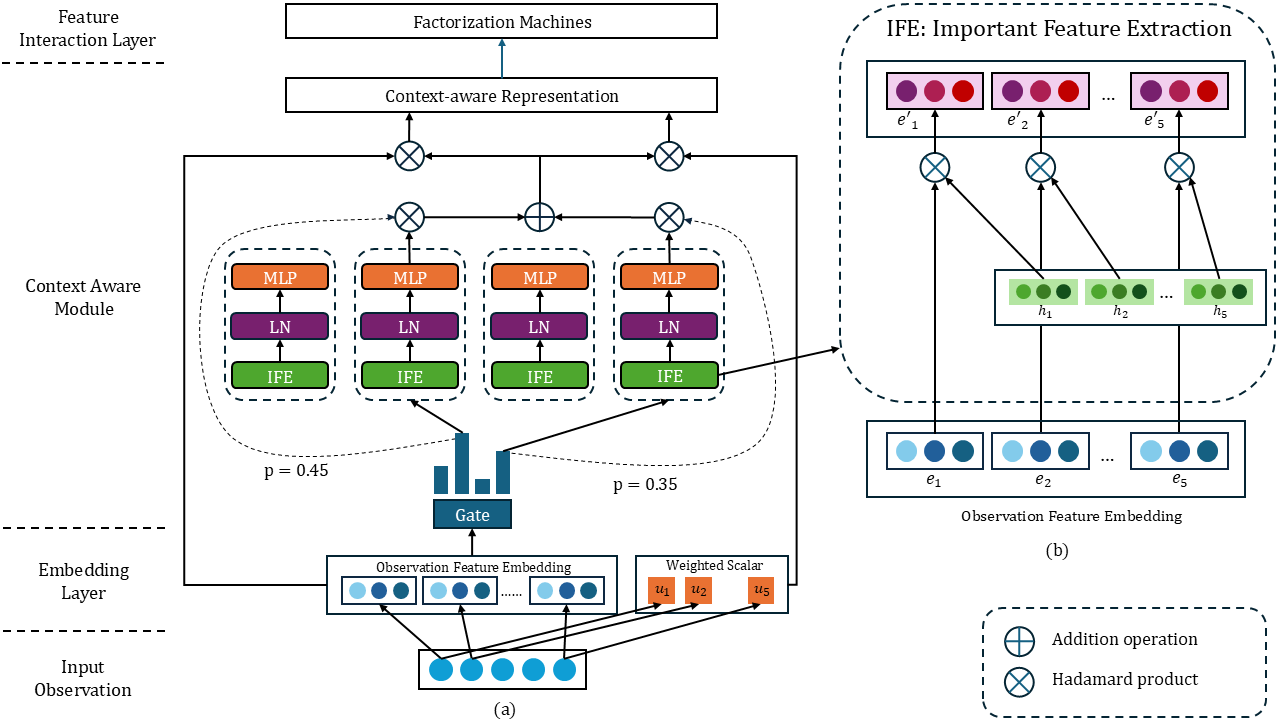
\includegraphics[width=\linewidth]{graphics/Overview Embedding.png}
%     \caption{(a) The overall architecture of Context Aware Module. (b) Important Feature Extraction.}
%     \label{fig:context_aware_module}
% \end{figure}
% % \vspace{1em}

\noindent\textbf{Embedding Layer:} From the initial joint observation $o_{i,j} = (i,j,\rho_{ij},\alpha_{ij})$, where $i$ and $j$ represent the sensor and target identifiers respectively, and $\rho_{ij}$ and $\alpha_{ij}$ are the real-valued distance and orientation angle formed between the sensor and the target, we will discretize these two values by segmenting the value ranges. Specifically, the discretized distance is defined as $\rho^*_{ij} =\lceil\frac{\rho_{ij}}{range\_size}\rceil $  and if $\rho^*_{ij}$ exceeds the environment size, it will be capped at that maximum value. The discretized angle is defined as $\alpha^*_{ij} =\lceil\frac{\alpha_{ij}}{range\_size}\rceil$. In this experiment, we choose $range\_size$ for $\rho$ and $\alpha$ to be $100$ and $15$, respectively.

Additionally, we introduce a status attribute $c_{ij}$ that indicates whether the target is within the detection range of the sensor based on $\rho_{ij}$ and $\alpha_{ij}$ from the observation. This attribute takes a value of 1 if the target is within range (i.e., \( \rho_{ij} < \rho_{\text{max}} \) and \( |\alpha_{ij}| < \alpha_{\text{max}} \)) and 0 if it is outside. Consequently, we obtain a discretized observation represented as $o^*_{ij} = (i,j,\rho^*_{ij},\alpha^*_{ij},c_{ij})$

Since these values are discretized, we employ a look-up embedding table to prevent sparse embeddings. Each feature $k$ of the observation is represented by an embedding vector $e_k\in \mathbb{R}^d$ , associated with a weighted scalar $u_k\in\mathbb{R}$, representing the influence or importance of that attribute. Thereby, the observation $o^*_{ij}$ of each sensor - target pair is represented as:  
\begin{equation*}
e = [e_1, e_2, \dots, e_5], \, u = [u_1, u_2, \dots, u_5]
\end{equation*}
where 5 is the number of features in the observation of each sensor - target pair.

% \vspace{1em}

\noindent\textbf{Context-Aware Module:} This model employs a Mixture of Experts(MoE) framework. 
The gating network uses a Multi Layer Perceptron (MLP) to generate weighted scalars $w_i$ for each expert $E_{i}$ . 
\begin{equation}
w = MLP(e)
\end{equation}
Then, we select the top $k$ largest weighted scalars from $w$ and their corresponding experts. The weighted scalars are normalized using the softmax function to avoid undesirable outputs.
\begin{equation}
w^*, E^* = topk (w), \,
w^*_{normalized} = Softmax(w^*)
\end{equation}

Each expert block $E^*_{i}$ is responsible for extracting the most significant features while eliminating irrelevant or noisy information. An extracting kernel $\mathbf{H} \in \mathbb{R}^{5 \times d}$ is utilized to perform this task, with the computation formula as follows: 
\begin{equation}
\mathbf{e}_i' = \mathbf{e}_i \otimes \mathbf{h}_i
\end{equation}
where \(\mathbf{h}_i\) is the \(i^{\text{th}}\) row in matrix \(\mathbf{H}\), \(\mathbf{e}_i\) is the \(i^{\text{th}}\) feature embedding.

Next, we apply Layer Normalization (LayerNorm) to standardize the output of the matrix. 
\begin{equation}
\mathbf{e}' = LayerNorm \left( \text{Concat} \left\{ \mathbf{e}'_i \mid i \leq 5 \right\} \right)
\end{equation}

The result is then passed through a Multi-Layer Perceptron (MLP) with a ReLU activation function, which generates a context-aware factor.
\begin{equation}
\mathbf{e}'^{(l+1)} = \text{ReLU}\left( \text{LayerNorm}\left( \mathbf{e}'^{(l)} \mathbf{W}^{(l)} + \mathbf{b}^{(l)} \right) \right)
\end{equation}
where \(\mathbf{W}^{(l)}\), \(\mathbf{b}^{(l)}\) denote the weight matrix and bias of the \(l^{\text{th}}\) layer. At the end of the stream, we derive the context-aware factor through a linear projection, mapping the intermediate vectors $\mathbf{e}'_L$ to the output of this expert block  $E^*_i\in\mathbb{R}^{1 \times 5} $

Following MoE framework, after obtaining the outputs from $k$ expert block. The outputs of these experts are aggregated as the weighted sum of the expert outputs, where the weight reflects the importance of each expert. The final result is a composite context-aware factor, which is then used in the subsequent layers.
\begin{equation}
m = \sum_{i} w^*_i(x) \cdot E^*_i
\end{equation}

\noindent\textbf{Reweighting Layer}: This layer adjusts the initial observation’s embedding vector by applying a context-aware factor from previous layers. This step produces a context-aware representation for the original observation. 
\begin{align}
e_i^* &= m_{i}\cdot e_i \\
u_i^* &= m_{i}\cdot u_i
\end{align}
where $ m_{i}$ indicates the weight for the $i^{\text{th}}$ feature.

% \vspace{1em}

\noindent\textbf{Feature Interaction:} Using the generated context-aware representations $e^*_i$ and $u^*_i$, a Factorization Machine algorithm is applied within this layer to compute a score $z$ for each sensor-target pair. This score captures the interaction strength between pairs, enabling efficient processing of contextual relations: 
\begin{equation}
z = u_0 + \sum_{i=1}^{n} u_i^* x_i + \sum_{i=1}^{n} \sum_{j=i+1}^{n} \langle e_i^* , e_j^* \rangle x_i x_j
\end{equation}
$\text{where } u_0 \text{ is the global bias, } x_i \text{ is the indicator of presentation of feature } i^{\text{th}}.$

% \vspace{1em}
% \begin{figure}[h]
%     \centering  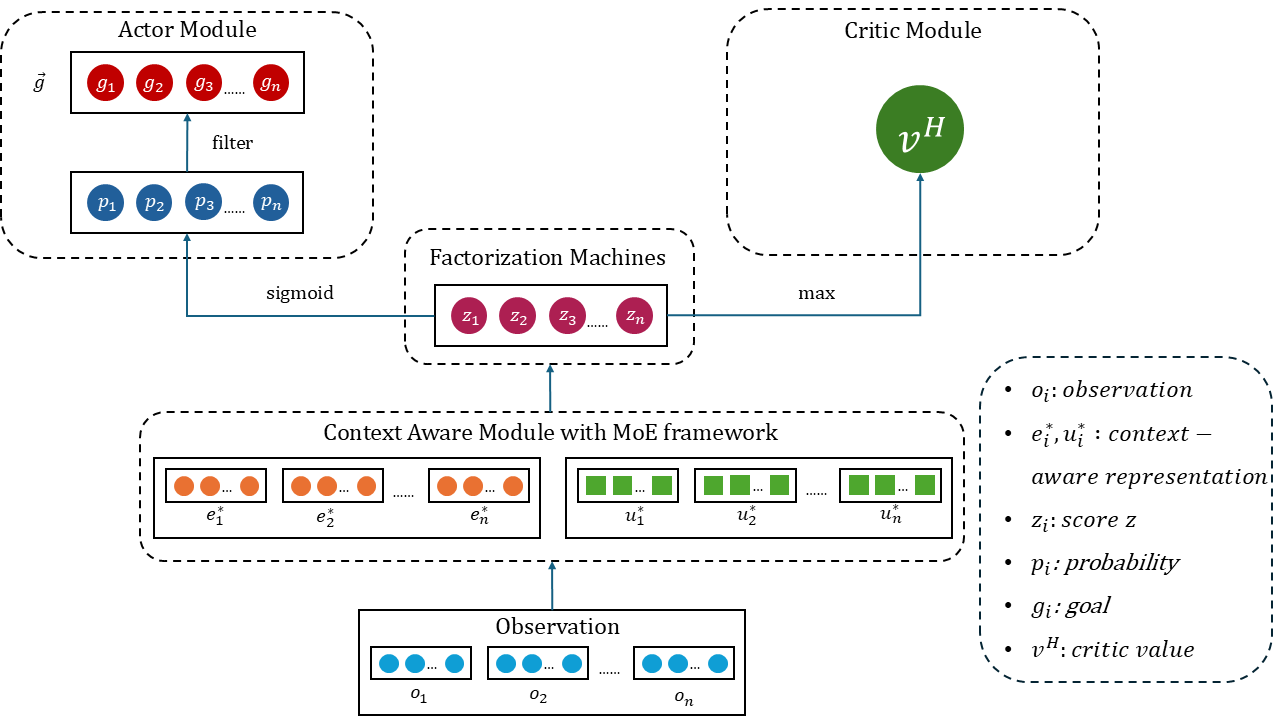
\includegraphics[width=\linewidth]{graphics/Integration.png}
%     \caption{Integrating Context-Aware Module with Actor-Critic Frameworks}
%     \label{fig:integration}
%     
% \end{figure}
\noindent\textbf{Actor:} The Actor module generates a goal map $\overset{\rightarrow}{g}\in\mathbb{N}^{n\times m} $ based on the interaction scores received from the Feature Interaction layer. It employs a sigmoid activation function to assign probabilities to each sensor-target pair. 
\begin{equation}
    prob_{ij} = sigmoid(z)
\end{equation}
where $prob_{ij}$ is the probability of $sensor_i$ - $target_j$ pair.
If the probability exceeds $0.5$, the corresponding sensor-target pair is designated as relevant for tracking (assigned a goal value of $1$); otherwise, it is marked as irrelevant (goal value of $0$). 

% \vspace{1em}

\noindent\textbf{Critic:} The Critic module evaluates the efficiency of the policy proposed by the Actor. This is achieved by learning a value that reflects the performance of the Actor's policy, which is subsequently used to update the parameters of the network layers to enhance policy effectiveness. Since the interaction scores from the Feature Interaction layer are indicative of the importance of each sensor-target pair, they are used as the basis for Critic's evaluation. Multiple methods can be applied to reduce the score vector into a scalar value for Critic, such as using the maximum score, summing, or averaging. In experimental trials, the best approach identified was to utilize the maximum score in the vector as the Critic's evaluation metric. 

% \vspace{1em}

The architecture of both the Actor and Critic components is more streamlined than in original approaches, as most computations are offloaded to preceding layers. The design primarily relies on Multi-Layer Perceptron (MLP) networks, reducing the number of learnable parameters compared to architectures that incorporate attention mechanisms. This leads to significant reductions in both training time and memory usage.

\subsection{Executor: Tracking Assigned Targets}
The executor, $\pi^{L}_i(a_i \mid o_i,g_i)$, gets its task goal $g_i$ from the coordinator, which includes a set of targets that need to be monitored. The executor's job is to track these targets independently and complete the tasks to earn its reward. 

Instead of directly passing the goal $g_i$ to executor $i$, the goal will be passed through a Goal-Condition Filter. This filter eliminates unnecessary information about irrelevant targets so that the executor will focus solely on the assigned targets. For instance, if $g_i$ is $[1,0,1]$ and the observation from sensor $o_i$ is $[o_{i,1}, o_{i,2}, o_{i,3}]$, after applying the filter, you will only keep the values $[o_{i,1}, o_{i,3}]$, discarding $o_{i,2}$.

During training, each executor's performance is judged based on a goal-conditioned reward $r_i$. This reward evaluates how closely the executor stays aligned with its assigned targets. We calculate each executor's reward by measuring the average relative angle between the observed targets and the executor's positions. 

The reward function is evaluated under two conditions: which are (a) the target $j$ is in the coverage range of the sensor $i$, i.e. $\rho_{i,j,t} < \rho_{\text{max}} \& |\alpha_{i,j,t}| < \alpha_{\text{max}}$; (b) target is outside of the range. 

\[
    r^L_{i,t} = \frac{1}{m_i} \sum_{j \in M_i} r_{i,j,t} - \beta \cdot cost_{i,t} 
\]
with
\[
\cdot r_{i,j,t} = 
    \begin{cases} 
    1 - \frac{|\alpha_{i,j,t}|}{\alpha_{\text{max}}}, & (a) \\ 
    -1, & (b)
    \end{cases} ,    cost_{i,t} = \frac{|\delta_{i,t} - \delta_{i,t-1}|}{z_{\delta}}
\]
Here $\alpha_{\text{max}}$ is the maximum viewing angle of the sensor, $\alpha_{i,j,t}$ is the relative angle from the front of the sensor to the target $j$, $M_i$ is a set of targets selected for the sensor $i$ according to $g_i$; $cost_{i,t}$ is the power consumption, measured by the normalized moved angle $\frac{|\delta_{i,t} - \delta_{i,t-1}|}{z_{\delta}}$; $\delta_i$ represents the absolute orientation of sensor $i$, the cost weight $\beta = 0.01$ and $z_{\delta}$ is the rotation angle, that is $5^\circ$ in original setting.

% \begin{figure}[h]
%     \centering  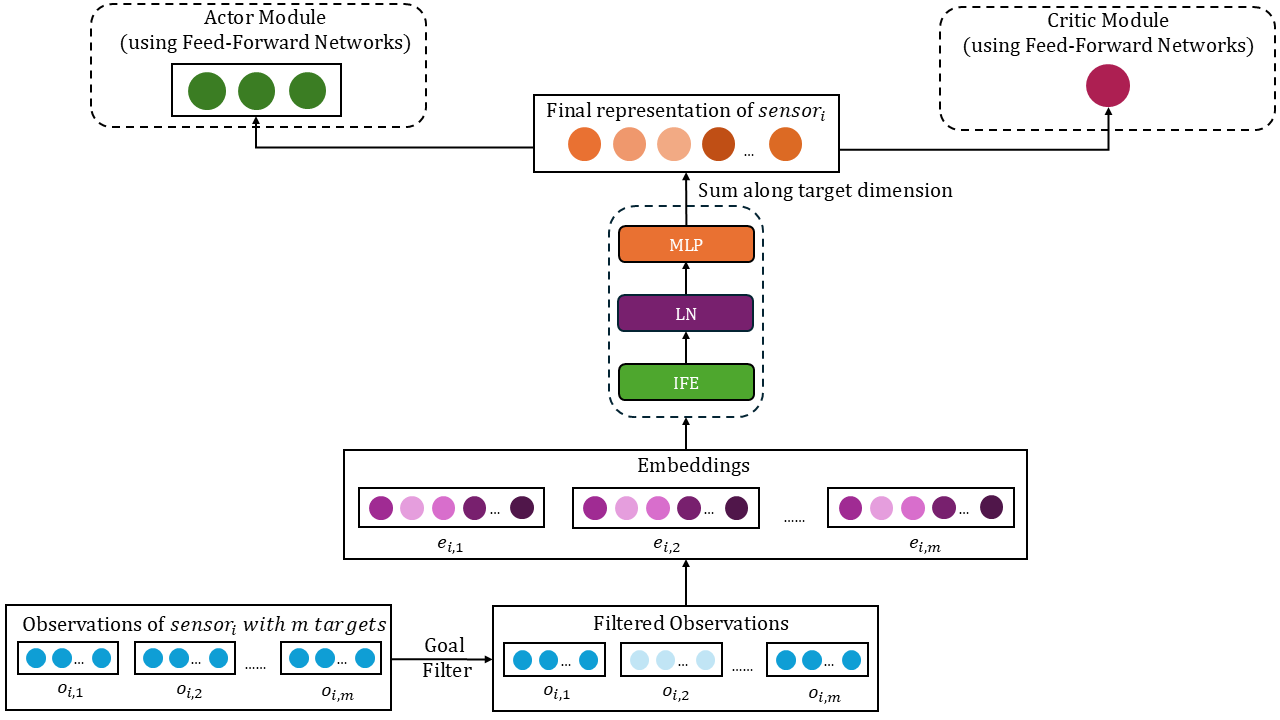
\includegraphics[width=\linewidth]{graphics/Executor.png}
%     \caption{The process of Executor with Actor-Critic Frameworks}
%     \label{fig:executor}
%     
% \end{figure}

The executor module is also designed as a deep neural network architecture that incorporates the actor - critic framework. The observations are first processed through a state encoder, which has been redesigned from its original attention-based implementation. While the original encoder utilized an Attention Layer, we replaced this component with a Context-Aware Module (CAM), omitting the Mixture of Experts (MoE) framework. This design is equivalent to setting the number of experts to 1 and the top-k selection to 1.

The Context-Aware Module follows the same process introduced in the Coordinator: (1) it performs important feature extraction, (2) applies Layer Normalization, and (3) passes the normalized features through a Multi-Layer Perceptron (MLP). Subsequently, before the features are forwarded to the Actor and Critic modules, the features of each sensor - target pair $ (sensor_i, target_j), \, j = 1, \dots, m $
$-$ where all pairs associated with the same $sensor_i$ across all $m$ targets $-$ are summed along the target dimension. The aggregated features are then processed through a Layer Normalization layer, resulting in the final representation of each sensor (executor).

The architectures of both the Actor and Critic modules have been simplified into single-layer Feed-Forward Network (FFN). The Actor network maps the extracted features to a probability distribution over possible actions, enabling policy optimization. Meanwhile, the Critic network outputs a scalar value representing the estimated state value, which helps evaluate the quality of the current policy. This simplified design reduces computational complexity while maintaining the effectiveness of the actor-critic framework.

\subsection{Training Strategy}
We employ a two-step training strategy, a widely adopted approach in hierarchical reinforcement learning, to enhance model stability. In the first step, we independently train the executor without the influence of the coordinator. The executor focuses solely on maximizing its local reward by targeting and capturing nearby objects within its visible range. This approach ensures the executor is not distracted by irrelevant or conflicting goals generated by the coordinator. Every $k$ time steps, the executor is assigned a goal based on the proximity between its current position and nearby targets. Specifically, targets located within the maximum coverage radius of sensor $i$ ($\rho_{ij,t}<\rho_{max}$) are selected as the goal $g_{i,t}$ for that sensor. This method fosters a more resilient tracking policy for the executor.

The second step involves training the coordinator, which can be done in two ways: either by training it independently from the pre-trained executor, using a random executor to receive and process goals, or by training it in conjunction with the pre-trained executor from step one. The latter approach allows the coordinator to rely on the learned behavior of the trained executor, which is already familiar with the environment, leading to improved performance over a stochastic executor. While both approaches yield similar results, training the coordinator independently takes longer to reach optimal performance. In contrast, training with the pre-trained executor is faster but requires additional memory to store the executor model.

In both training approaches, the coordinator updates the observations and generates new goals for the executors every $k$ steps, aligning with the time steps of the executors. The executors then act on these goals, and after $k$ steps, they transfer their updated observations back to the coordinator to receive new objectives, thereby maintaining a continuous and efficient training process.

In our experiments, we fixed $k = 10$, and both the coordinator and executor were trained using the A3C algorithm, a hybrid of RL and deep learning techniques. Each component leveraged a distinct architecture, ensuring that the models could focus on their respective tasks independently and reducing interference between the two components while ensuring optimal performance once integrated.

%Given the \gls{aoi} of size $W \times H$. The area is divided into $n_{cell}$ cells of size $w_{cell} \times h_{cell}$. Consequently, there are $n_{cell}$ targets $t_1, t_2, \dots, t_{n_{cell}}$, each of which is located at the center of a cell. Assume that the heterogeneous sensor set $S = \{s_1, s_2, \dots, s_{|S|}\}$ where each sensor belongs to either one of the two predefined types with sensing range $R_1$ and $R_2$ is deployed in the \gls{aoi}. Here, we define the term $r_{cov}$ which shows the coverage ratio in the \gls{aoi} (i.e., the ratio of targets considered covered) \cite{Li2009}:
%\begin{equation}
   % r_{cov} = n^+_T / n_{cell}.
    %\label{eq:rcov}
%\end{equation}
%where $n^+_T$ denotes the number of targets accepted as covered (based on $TH_{cov}$). Our objective is maximizing $r_{cov}$ while minimizing $|S|$ by finding locations of all heterogeneous sensors in $S$. $|S|_{min}$ and $|S|_{max}$ are calculated as in \eqref{eq:|S|min} and \eqref{eq:|S|max}. The problem formulation is described below:

%\textbf{Maximize:} $r_{cov}$ while \textbf{Minimize:} $|S|$

%\textbf{Subject to:}
%\begin{alignat}{3}
   % & |S|_{min} \ & \leq & \ |S| \ & \leq & \ |S|_{max}, \\
    %& x^{(L)}_s \ & \leq & \ x_s \ & \leq & \ x^{(U)}_s \quad \forall s \in S, \\
    %& y^{(L)}_s \ & \leq & \ y_s \ & \leq & \ y^{(U)}_s \quad \forall s \in S.
%\end{alignat}

%This is a multi-objective problem. In this paper, we leverage \gls{hs} to solve it by constructing a good fitness function to direct the search process to achieve both objectives simultaneously. The applications of this problem in real life are elaborated in the next section.



\section{Experiments}
\label{sec:experiments}
In this experiment, we conduct a comparative analysis of our proposed model to investigate the following research questions:

\noindent\textbf{RQ1:} How does our proposed model compare to the baseline model in terms of coverage performance in a small-scale HiT-MAC scenario for Directional Sensor Networks (DSNs)?

\noindent\textbf{RQ2:}  How does our proposed model perform relative to the baseline model in a large-scale simulated environment with a reduced sensor detection range, representing a more complex and resource-constrained DSN setting?

\noindent\textbf{RQ3:} What is the impact of varying the number of experts within the Mixture of Experts (MoE) framework on the coverage performance of the proposed model in the large-scale scenario?
% against the baseline model in two distinct simulated environments, both of which are designed to replicate the target coverage challenge in real-world Directional Sensor Networks (DSNs). The first environment corresponds to the small-scale HiT-MAC scenario, which was originally evaluated in the foundational paper. The second environment is a large-scale scenario developed specifically for this evaluation, consisting of a sensor population and target range spanning from 50 to 100 units, but with a reduced sensor detection range to assess the performance of both models in a more complex, resource-constrained setting. In the large-scale environment, we further perform an ablation study to investigate the impact of varying the number of experts within the Mixture of Experts (MoE) framework employed in our model, thereby validating the contribution of expert diversity in enhancing coverage performance.
\subsection{Environments}
The evaluation environment is a two-dimensional bounded area. At the start of each episode, the $n$ sensors are randomly deployed, while the $m$ targets are initialized at arbitrary locations. These targets move with random velocities and follow unpredictable trajectories throughout the episode. This setup allows for a dynamic simulation of real-world target tracking and coverage scenarios within the constraints of Directional Sensor Networks.

\textbf{Observation Space:} At each time step, the observation $o_i$ for sensor $i$ is constructed based on the sensor-target relationships, denoted as $o_i = (o_{i,1}, o_{i,2}, \dots, o_{i,m})$, where $o_{i,j} = (i, j, \rho_{ij}, \alpha_{ij})$ represents the spatial relationship between sensor $i$ and target $j$ in a polar coordinate system with sensor $i$ positioned at the origin. Specifically, $i$ and $j$ are the unique identifiers for the sensor and target, respectively, while $\rho_{ij}$ and $\alpha_{ij}$ represent the absolute distance and relative angle from sensor $i$ to target $j$. In the case of the coordinator within the HiT-MAC framework, the joint observation is represented as $\overset{\rightarrow}{o} = (o_1, o_2, ..., o_n)$, aggregating the observations from all $n$ sensors.

\textbf{Action Space:} The primitive action space consists of three discrete actions: \textit{TurnRight}, \textit{TurnLeft}, and \textit{Stay}. The \textit{TurnRight} and \textit{TurnLeft} actions adjust the sensor's absolute orientation $\delta_i$ incrementally by 5 degrees per step, i.e., \textit{Right}: $\delta_{i,t+1} += 5^\circ$, \textit{Left}: $\delta_{i,t+1} -= 5^\circ$. In the HiT-MAC framework, the coordinator uses a goal map $\tilde{g}$, which is an $n \times m$ binary matrix, where $g_{i,j}$ indicates whether target $j$ has been assigned to sensor $i$ (0: No, 1: Yes). Each row of the matrix corresponds to the target assignment for each individual sensor.
\subsection{Experiment Scenarios}
To evaluate the efficiency of the proposed model compared to the baseline, we conducted experiments in two distinct environmental scenarios, each designed to rigorously assess sensor coverage capabilities in dynamic target tracking tasks

\textbf{Scenario 1: Small-Scale Environment:} The first scenario replicates a small-scale environment from the original study, employing $n = 4$ directional sensors with fixed locations and limited orientations, tasked with tracking $m = 5$ mobile targets. This setup serves as a baseline for performance comparison, providing a controlled environment to benchmark coverage efficiency.

\textbf{Scenario 2: Large-Scale Environment:} The second scenario introduces a large-scale environment structured as a $10 \times 10$ grid, designed to test the model’s scalability and adaptability. In this environment, sensor placement is probabilistic, with each grid cell assigned a uniform probability of sensor deployment. A threshold probability of 50\% determines the overall sensor distribution, resulting in a total of 50 sensors and 60 targets across the grid.

The probabilistic model guiding sensor placement effectively reflects
the inherent uncertainties associated with real-world sensor positioning. To further refine the experimental setup, the radius of each sensor was
adjusted to ensure that the circular detection area produced by a sensor is
confined to a single grid cell. This modification facilitates enhanced control
over sensor coverage, thereby more accurately simulating conditions where
sensors possess limited detection ranges and must be strategically oriented
to optimize coverage within the environment.
\subsection{Hyper-parameters Setting}
The hyper-parameters for the A3C framework, Coordinator and Executor networks are detailed in Table 1
\begin{table}[ht]
\caption{Hyper-parameters Setting.}
\centering
\footnotesize
\begin{tabular}{cccc}
\hline
\textbf{Hyper-parameters} & \textbf{\#} & \textbf{Description} \\
\hline
hidden units & 128 & the \# of hidden units for all layers \\

hidden layers & 2 & the \# of hidden layers in MLP component\\

training episodes & 50k & maximum training episodes \\

episode length & 100 & maximum time steps per episode \\

discount factor & 0.9 & discount factor for rewards \\

entropy weight & 0.01 & parameter for entropy regularization \\

learning rate & 5e-4 & learning rate for all networks \\

workers (small) & 10 & the \# of workers of the A3C framework in Scenario 1 \\

workers (large) & 40 & the \# of workers of the A3C framework in Scenario 2 \\

update frequency & 20 & the master network updates every \# steps in A3C \\
\hline
\end{tabular}
\end{table}
\subsection{Results}

We use the coverage rate to evaluate the performance of each model. This metric quantifies the percentage of targets successfully covered by sensors relative to the total number of targets.
\subsubsection{Scenario 1: Small-Scale Environment (RQ1)}
% \begin{figure}[h]
%     \centering  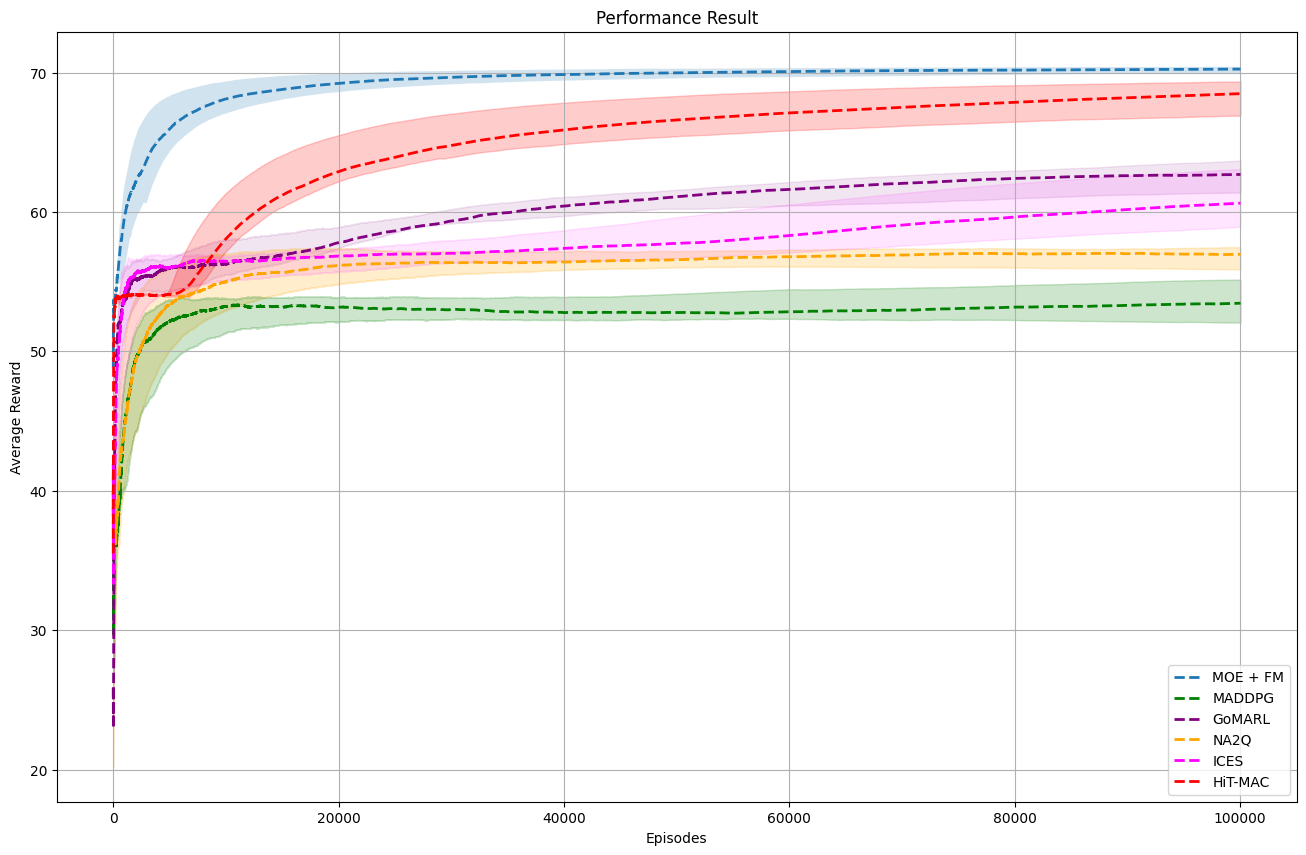
\includegraphics[width=\linewidth]{graphics/Results_final.png}
%     \caption{The learning curves of all methods}
%     \label{fig:result}
%     
% \end{figure}
As illustrated in Figure 5, our proposed model demonstrates significant superiority over the baseline model in achieving higher coverage rates (\%) over the course of approximately 100,000 training episodes. Our model not only converges to optimal performance more rapidly but also maintains consistently higher performance throughout the training process.

Specifically, our model achieves a coverage rate of approximately 69\% by as early as 20,000 episodes, significantly surpassing the baseline model. By the conclusion of training, it stabilizes at an impressive coverage rate of around 71\%, indicating its robustness and effectiveness. In contrast, the original HiT-MAC model exhibits a much slower progression, with prolonged stagnation at approximately 55\% coverage for a significant portion of the early training episodes. This disparity highlights the efficacy of our approach in consistently progressing toward optimal coverage rates, in stark contrast to the oscillatory behavior exhibited by the original model.

The performance of our model can be attributed to the use of Factorization Machines (FMs), which excel in explicitly modeling pairwise feature interactions. This capability is particularly advantageous in the context of directional sensor coverage, where interactions among sensor direction, range, and orientation are critical to optimizing overall coverage. By providing a direct representation of these relationships, FMs are able to effectively capture influential feature combinations, enabling faster and more precise learning.

On the other hand, the attention mechanisms employed in the baseline model implicitly capture feature interactions, focusing primarily on the relative importance of individual features rather than explicitly modeling their pairwise relationships. While this approach has its merits, it falls short in scenarios where the understanding of direct interactions between features is essential. This limitation leads to slower learning and suboptimal coverage rates in the baseline model, further emphasizing the advantages of our proposed approach.

% Furthermore, we evaluated the training efficiency of both models in terms of frame rate, measured in frames per second (FPS). Our model achieves a frame rate of approximately 95-100 FPS per episode, whereas the original model operates at approximately 75-80 FPS. This notable difference indicates that our model necessitates a reduced training time compared to the original model.

% This enhanced efficiency can be attributed to the reduced complexity of our model architecture, which primarily utilizes a Feed Forward Network, resulting in fewer parameters to optimize during the learning process. In comparison, the original model employs an Attention Module, which, while effective, incurs a substantial computational burden due to its larger parameter space. Although the drawbacks of the Attention Module may not be immediately evident in a small-scale environment, they become significantly pronounced when scaling to larger environments, as explored in the subsequent scenario. The increase in model size in larger environments leads to an exponential rise in the number of parameters, substantially augmenting the model's overall capacity and complexity.

\subsubsection{Scenario 2: Large-Scale Environments (RQ2)}
\begin{table}[ht]
\centering

\begin{tabular}{lc} % 'l' for left-align, 'c' for center-align
\hline
\textbf{Methods} & \textbf{Coverage rate(\% ) } \\
\hline
MADDPG & 18.05 \\
NA2Q & 18.75 \\
GoMARL   & 20.54 \\
ICES   & 18.82 \\
HiT-MAC   & - \\
\hline
\textbf{Ours} & \textbf{26.64} \\
\hline
\end{tabular}
\caption{Comparative results of different methods (n=50\&m=60). HiT-MAC was  unable to execute due to excessive memory demands}
\end{table}


In this large-scale environment, the original model faced significant resource constraints, which rendered it unable to execute due to excessive memory demands. Specifically, employing an Attention Module to manage 3,000 sensor-target pairs required an immense amount of memory to store all potential configurations and intermediary states. Although our experimental setup provided a computing environment with ample memory resources, the original model's memory requirements surpassed the available RAM capacity, making its execution infeasible.

In contrast, our proposed model, designed with a simpler and more efficient architecture, demonstrated considerably lower memory consumption, even in this demanding large-scale context. We employed a coordinated training strategy that utilized parallel execution of the coordinator and executor components, enabling the model to handle computationally intensive tasks more effectively. By integrating these components during the inference stage, we achieved an average coverage rate of 27.41\%, with peak performance in a single episode reaching approximately 31.1\%.

To evaluate the effectiveness of our approach, we calculated the coverage area as a percentage of the environment covered by the sensor range relative to the total area. The results revealed that the sensors achieved approximately 20\% coverage. This coverage is notable given the inherent limitations imposed by sensor range and environment scale. Our strategic learning methodology, which balances computational efficiency and sensor utilization, allowed the model to achieve superior performance compared to results based solely on the sensor range. This demonstrates the effectiveness of our approach in optimizing resource use while maintaining high coverage rates in large-scale scenarios.

\subsubsection{Ablation Study on the Number of Experts in Mixture of Experts (MoE) Frameworks (RQ3)}
We conducted an ablation study to assess the impact of the number of experts and the number of top experts ($k$) within the context of both small-scale and large-scale environments. The results indicated that performance gains associated with an increased number of experts highlight the significance of having a diverse set of experts in the MoE framework.
\begin{table}[ht]
\centering
\caption{Results of different $k$ and num\_experts settings.}
\begin{tabular}{cc|cc|cc}
\hline
\textbf{k} & \textbf{num\_experts} & \multicolumn{2}{c|}{\textbf{large-scale env.}} & \multicolumn{2}{c}{\textbf{small-scale env.}} \\ 
\cline{3-6}
& & \textbf{BEST} & \textbf{AVG} & \textbf{BEST} & \textbf{AVG} \\ 
\hline
1 & 1 & 30.43 & 25.91 & 86.79 & 69.74 \\ 
1 & 2 & 31.15 & 26.36 & 86.94 & 69.88 \\ 
1 & 4 & 31.02 & 26.45 & 87.11 & 69.92 \\ 
2 & 4 & 31.17 & 26.64 & 87.95 & 70.24 \\ 
\hline
\end{tabular}
\end{table}

Increasing the number of experts (\text{num\_experts} = 4) consistently enhances performance compared to utilizing a single expert. This aligns with the expectations of MoE models, where a larger number of experts contributes to greater specialization and diversity. More experts enable the model to specialize and select more optimal functions tailored to specific tasks, resulting in improved performance. In scenarios with \text{num\_experts} = 1, the lack of specialization forces the single expert to generalize across all tasks, which can lead to suboptimal outcomes. In contrast, with four experts, the framework can effectively route inputs to the most relevant expert, yielding better performance.

In the small-scale environment, the impact of increasing both \text{num\_experts} and $k$ is more pronounced. With a relatively simpler task or smaller environment, the model benefits more from the additional expertise. The selection of multiple experts ($k = 2$) in this setting leads to noticeable improvements in performance. This is likely due to the increased ability of the MoE framework to introduce more specialized knowledge, which compensates for the limitations of smaller environment. In the small-scale case, the increase in expert selection brings out the complementary capabilities of each expert, resulting in a broader range of knowledge and better task-specific optimization.

However, in the large-scale environment increasing the number of top experts ($k$) does not appear to confer significant benefits beyond a certain threshold. This may occur because the selected experts lack sufficient distinction or specialization, resulting in overlapping knowledge and skills. When experts do not differentiate significantly in their functions, adding more experts fails to provide unique insights or enhance predictive accuracy.

The fundamental principle of the Mixture of Experts framework is to route specific inputs to the most suitable experts, with each expert ideally addressing different facets of the problem space. Nevertheless, when multiple experts share similar functions or knowledge, the selection of several experts can lead to redundancy, thereby diminishing the advantages of employing a larger expert pool.

\section{Conclusion}













\end{document}
